\documentclass{article}
\usepackage{graphicx}
\usepackage{subfig}
\usepackage{cite}
\usepackage{float}

\begin{document}
\title{Applying Information Theory to a Fully Recurrent Neural Network}
\author{Stefan Ivanovic, Benjamin Kha, Vignesh Muruganantham}
\date{April 15 2018}
\maketitle{}

\section{Abstract}

In this paper, we use information theory to analyze a fully recurrent neural network. The neural network is trained to predict daily temperatures from weather data in the past several days. We analyze if a natural structure develops in the network (since there is very little structure imposed on a fully recurrent neural network). To do this, we form graphs of the information flow in the network and develop an ranking algorithm to help analyze it�s structure. We find only slight traces of a structure developing on the network. We also analyze how information theory related statistics can be used as learning indicators. Additionally, we look at whether the information bottleneck principle appears to apply to fully recurrent neural networks (as it has been shown to apply to feed forward neural networks).  We find no indication that the information bottleneck principle still applies.

\section{Background Information and Related Work}

This paper assumes a knowledge of basic Information Theory. Specifically, we assume knowledge of entropy (for continuous variables), mutual information (for continuous variables), and time delayed mutual information (for continuous variables). For a refresher on this topic, I highly recommend chapter 2 of 'Information Theory for Analyzing Neural Networks''. Recall that the mutual information for two continuous random variables $X, Y$ is defined as

\[
  I(X;Y) = - \int \int f(x, y) \log_2 \frac{f(x, y)}{f(x) f(y)} dx dy
\]

Of course, the probability densities of the random variables we wish to study are not known to us, so we use nonparametric methods to estimate this quantity (and all other information theoretic quantities in this paper). For more information on how we estimate these quantities, see Kraskov [10].

We also utilize TSE complexity, however, not having a precise knowledge of how TSE complexity is calculated should not hinder your understanding of the paper. For all of our information theoretic analyses we use the entropy estimator toolbox from https://www.isi.edu/~gregv/npeet.html. For our fully recurrent neural network we use the network of https://github.com/moaljazaery/RRN-Weathre\_ Forcasting (''Weathre'' is not a typo).

Information theory has been a very successful tool for understanding neural networks. One important example of this is the application of the information bottleneck principle to feed forward neural networks. In ''Opening the black box of Deep Neural Networks via Information'' the mutual information of each layer of their feed forward neural network with the inputs and ground truth outputs was calculated during training. Analyzing these results (as well as the gradient) showed that training was split into two phases. In the first phase, the mutual information with the input and output both increased as one would naturally expect. In the second phase, the mutual information with the input significantly decreases and the mutual information with the output slightly decreased. In their paper, they described this second phase as learning to ''forget'' information about the input, in order to become more general (and less likely to over fit). This relates to the information bottleneck principle, since the network appears to be �trying� to become more like the �perfect� network which keeps the minimal amount of information about the input which is sufficient for predicting the output. In our paper, we analyze if these results generalize to our fully recurrent neural network.

In the paper ''Information Theory for Analyzing Neural Networks'', information theory was applied to recurrent neural networks (as well as feed forward neural networks);  However, the analysis done was specifically fit to a very simple controller network. In our paper, we analyze a larger (than their tiny example) fully recurrent neural network, designed for weather prediction. In �Information Theory for Analyzing Neural Networks�, it was found that information theory based statistics can help indicate that the network is learning before the error greatly decreases. This can potentially be very useful in cases where you would want to know if the network is successfully learning before waiting for the error to significantly decrease. In this paper, these indicators of learning are called ''learning indicators'' and were shown to be very effective for our network.

\section{Motivation}

One of the largest goals in the field of machine learning is to truly understand the neural networks rather than treating them as a partially understood black box. In my opinion, one of the best ways to understand neural networks is to look at the case where very little structure is imposed on the network, and consequently the network is free to develop almost all its structure naturally during training. Therefore, I believe analyzing fully recurrent neural networks (in which all hidden neurons have connections to all other hidden neurons) is an excellent place to start. Additionally, Information Theory has generally been the most fruitful method for understanding neural networks. Therefore, in this paper, we choose to apply information theory to a fully recurrent neural network.

After choosing to analyze fully recurrent neural networks via Information Theory, the first question that arises is ''should we apply traditional information theoretic techniques used on feed forward neural networks to our recurrent neural network or design new techniques for recurrent neural networks?''. Noting that the second option is incredibly ambitious (possibly overly) and risky, yet potentially more powerful, we decided to do both. When it comes to utilizing known methods, we decided to apply the information bottleneck principle and learning indicators (which in ''Opening the black box of Deep Neural Networks via Information'' are not explicitly called ''learning indicators'', but are explained to indicate learning). When it comes to designing new methods, we invented the ''information flow graph'' and ''neuron ranking algorithm''. I believe the information flow graph contains an absolute plethora of information useful for understanding how structure develops on neural networks, however, it is extremely difficult to extract this information. Our ranking algorithm was our most successful attempt at extracting information from the information flow graph, and yielded very encouraging results.

\section{Creating the Information Flow Graph}

Our goal in creating an information flow graph is to create a directed graph with neurons as vertices, and directed edges which best represent how information flows from each neuron to the next. The most obvious approach is to just calculate the mutual information between each neurons, and to create an edge connecting two neurons if this mutual information is above some cut off. However, this has multiple problems. The most obvious problem is that this would create an undirected graph, however, that can be fixed by just replacing regular mutual information with time delayed mutual information. The greater flaw is that this would create false edges representing incorrect information flow. This is best explained through an example. If neuron A greatly  influences neuron B and neuron C, then their will be a high mutual information between B and C because they both have a high mutual information with A. Therefore, using mutual information directly would produce an edge between B and C, despite the fact that no information flows between B and C. Using time delayed mutual information technically fixes this problem (for this specific example), however, it also has very similar problems (which require slightly more complicated examples to show which will not go into). The solution is simply to look at the time delayed mutual information minus the mutual information, which we will define as the information flow between two neurons. This calculates how much each neuron directly influences the other neurons and removes the effect of two neurons having a high mutual information without actually influencing each other.

Using this method to calculate the information flow between neurons, we can create an information flow graph by including an edge from neuron A to neuron B if the information flow from neuron A to neuron B is above some threshold. We get the following, rather chaotic looking, graphs. The difference between the graphs is just the threshold we choose for how high the information flow must be in order to add an edge to the graph. The numbers on the neurons just allow you to look at the same neuron in different graphs.

\begin{figure}[H]
\centering
\noindent
\subfloat[Threshold=0.006]{{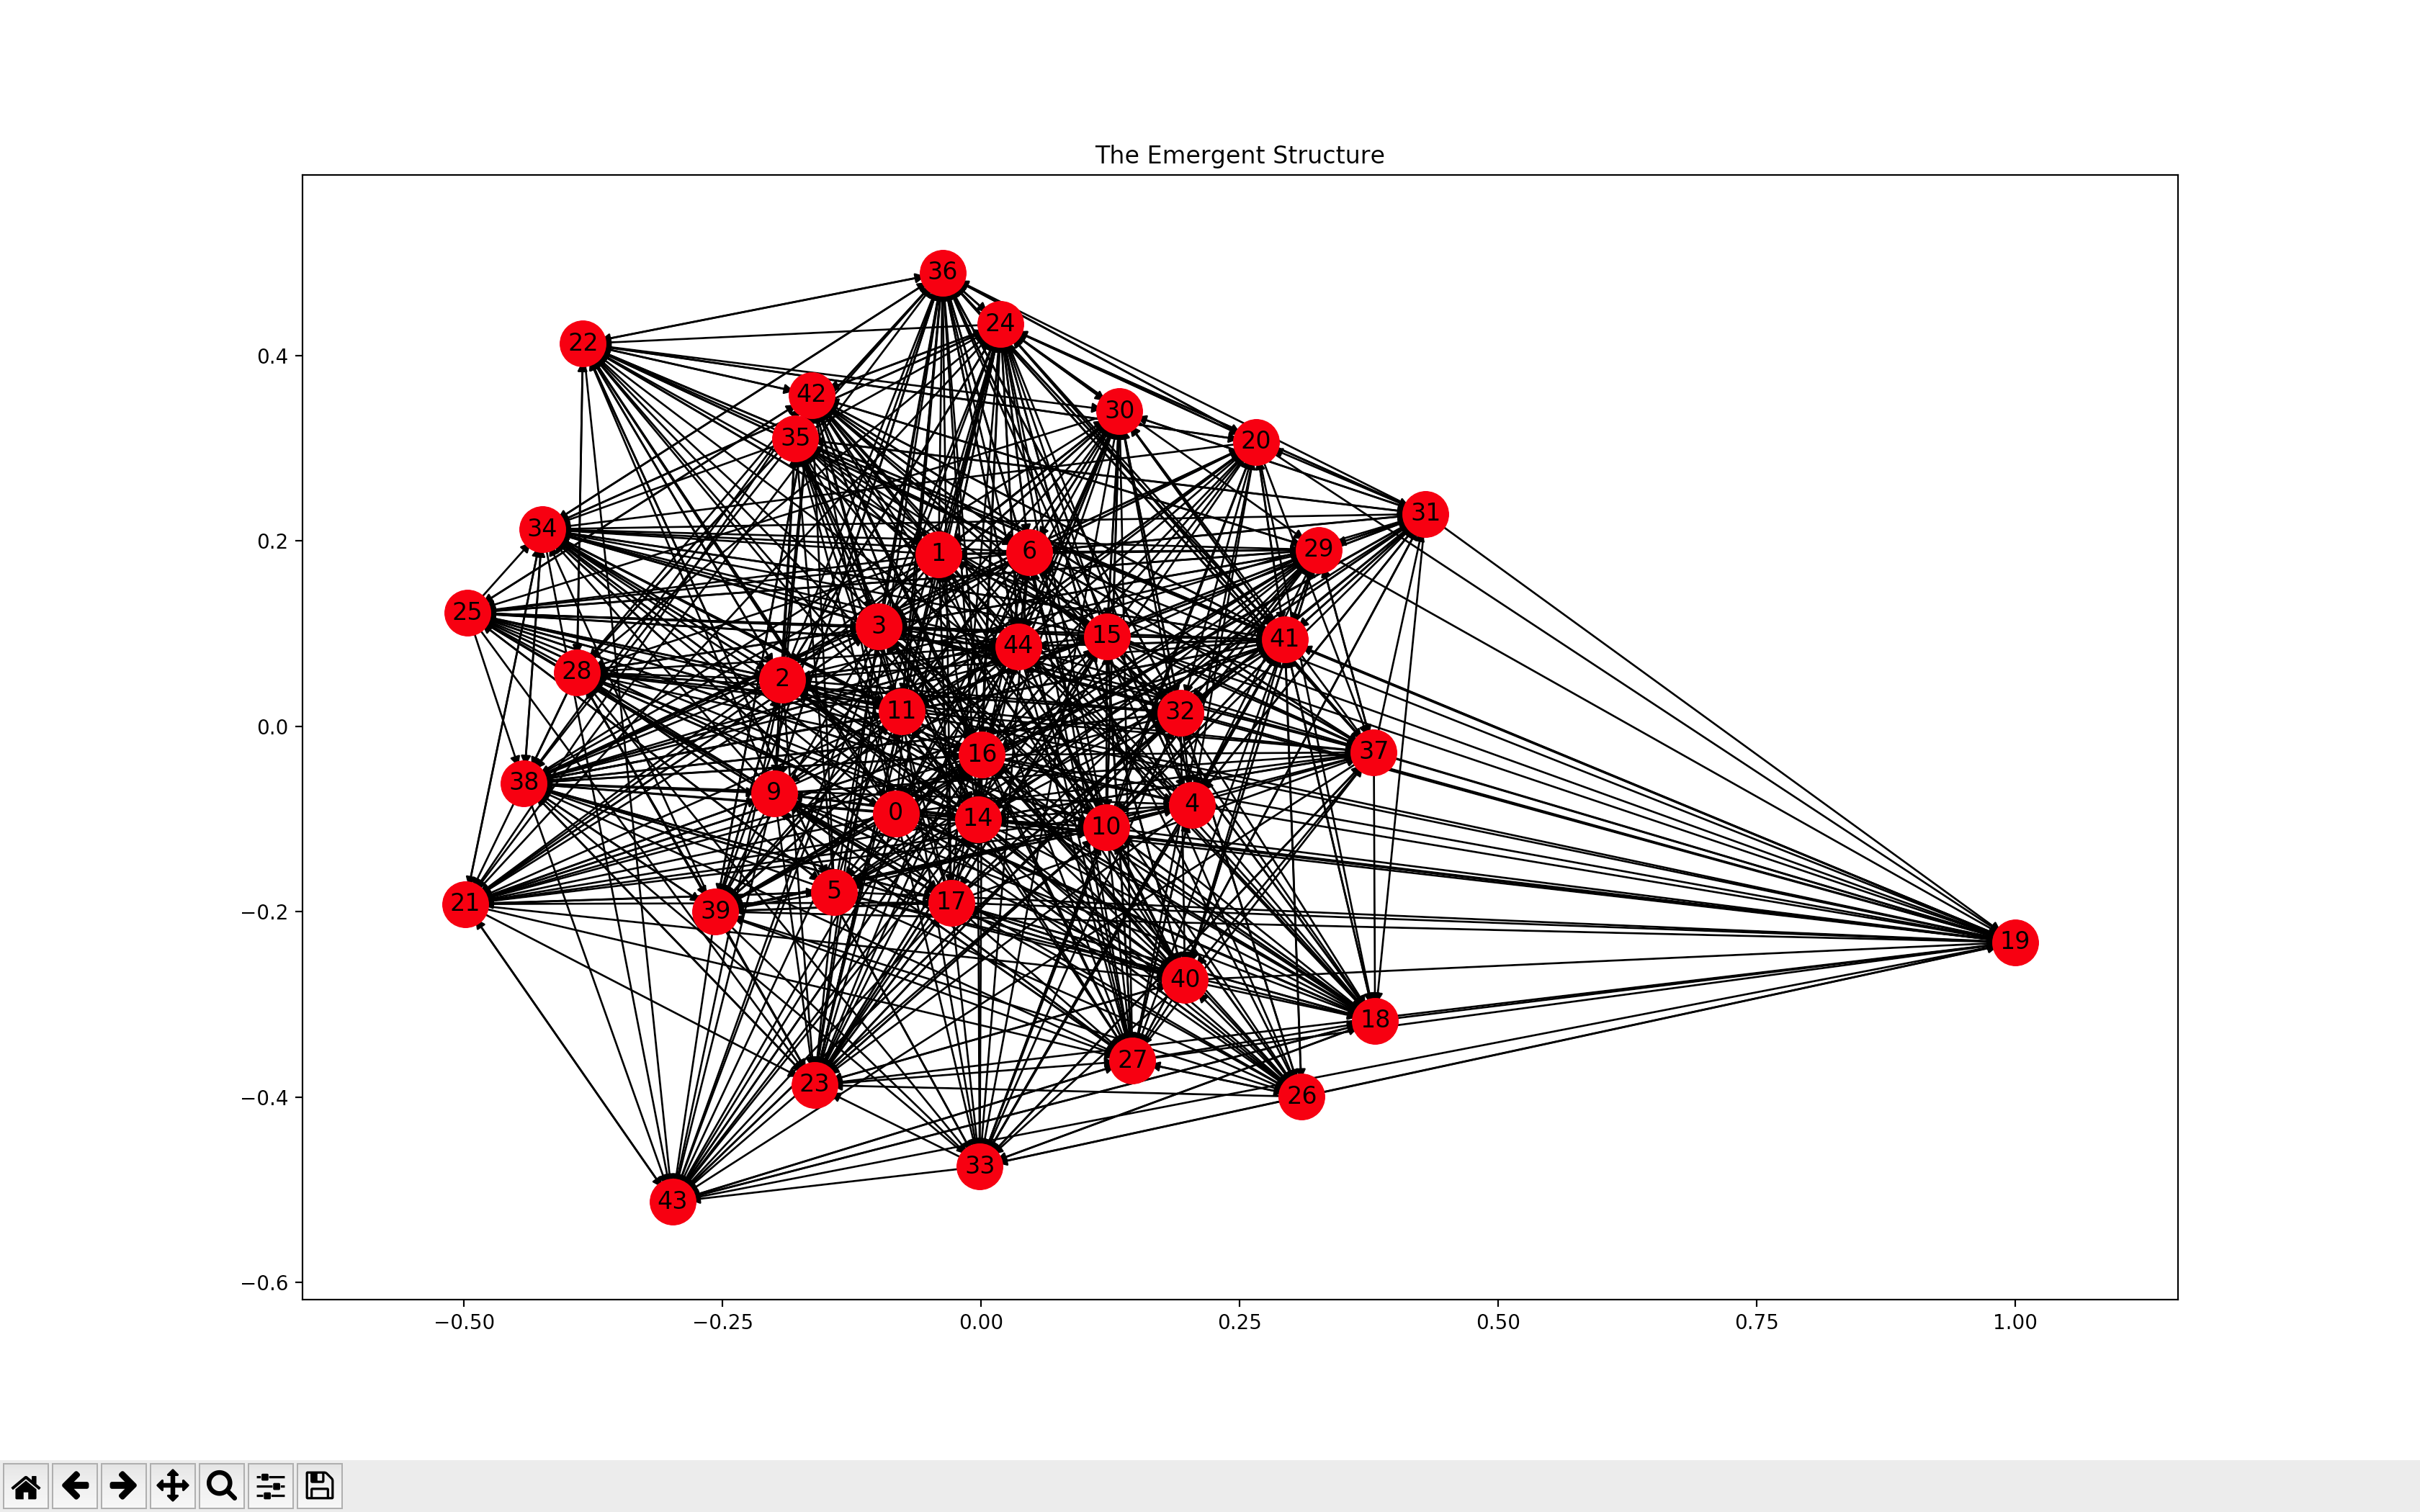
\includegraphics[width=5.8cm]{RNN_Images/7_006} }}%
\subfloat[Threshold=0.04]{{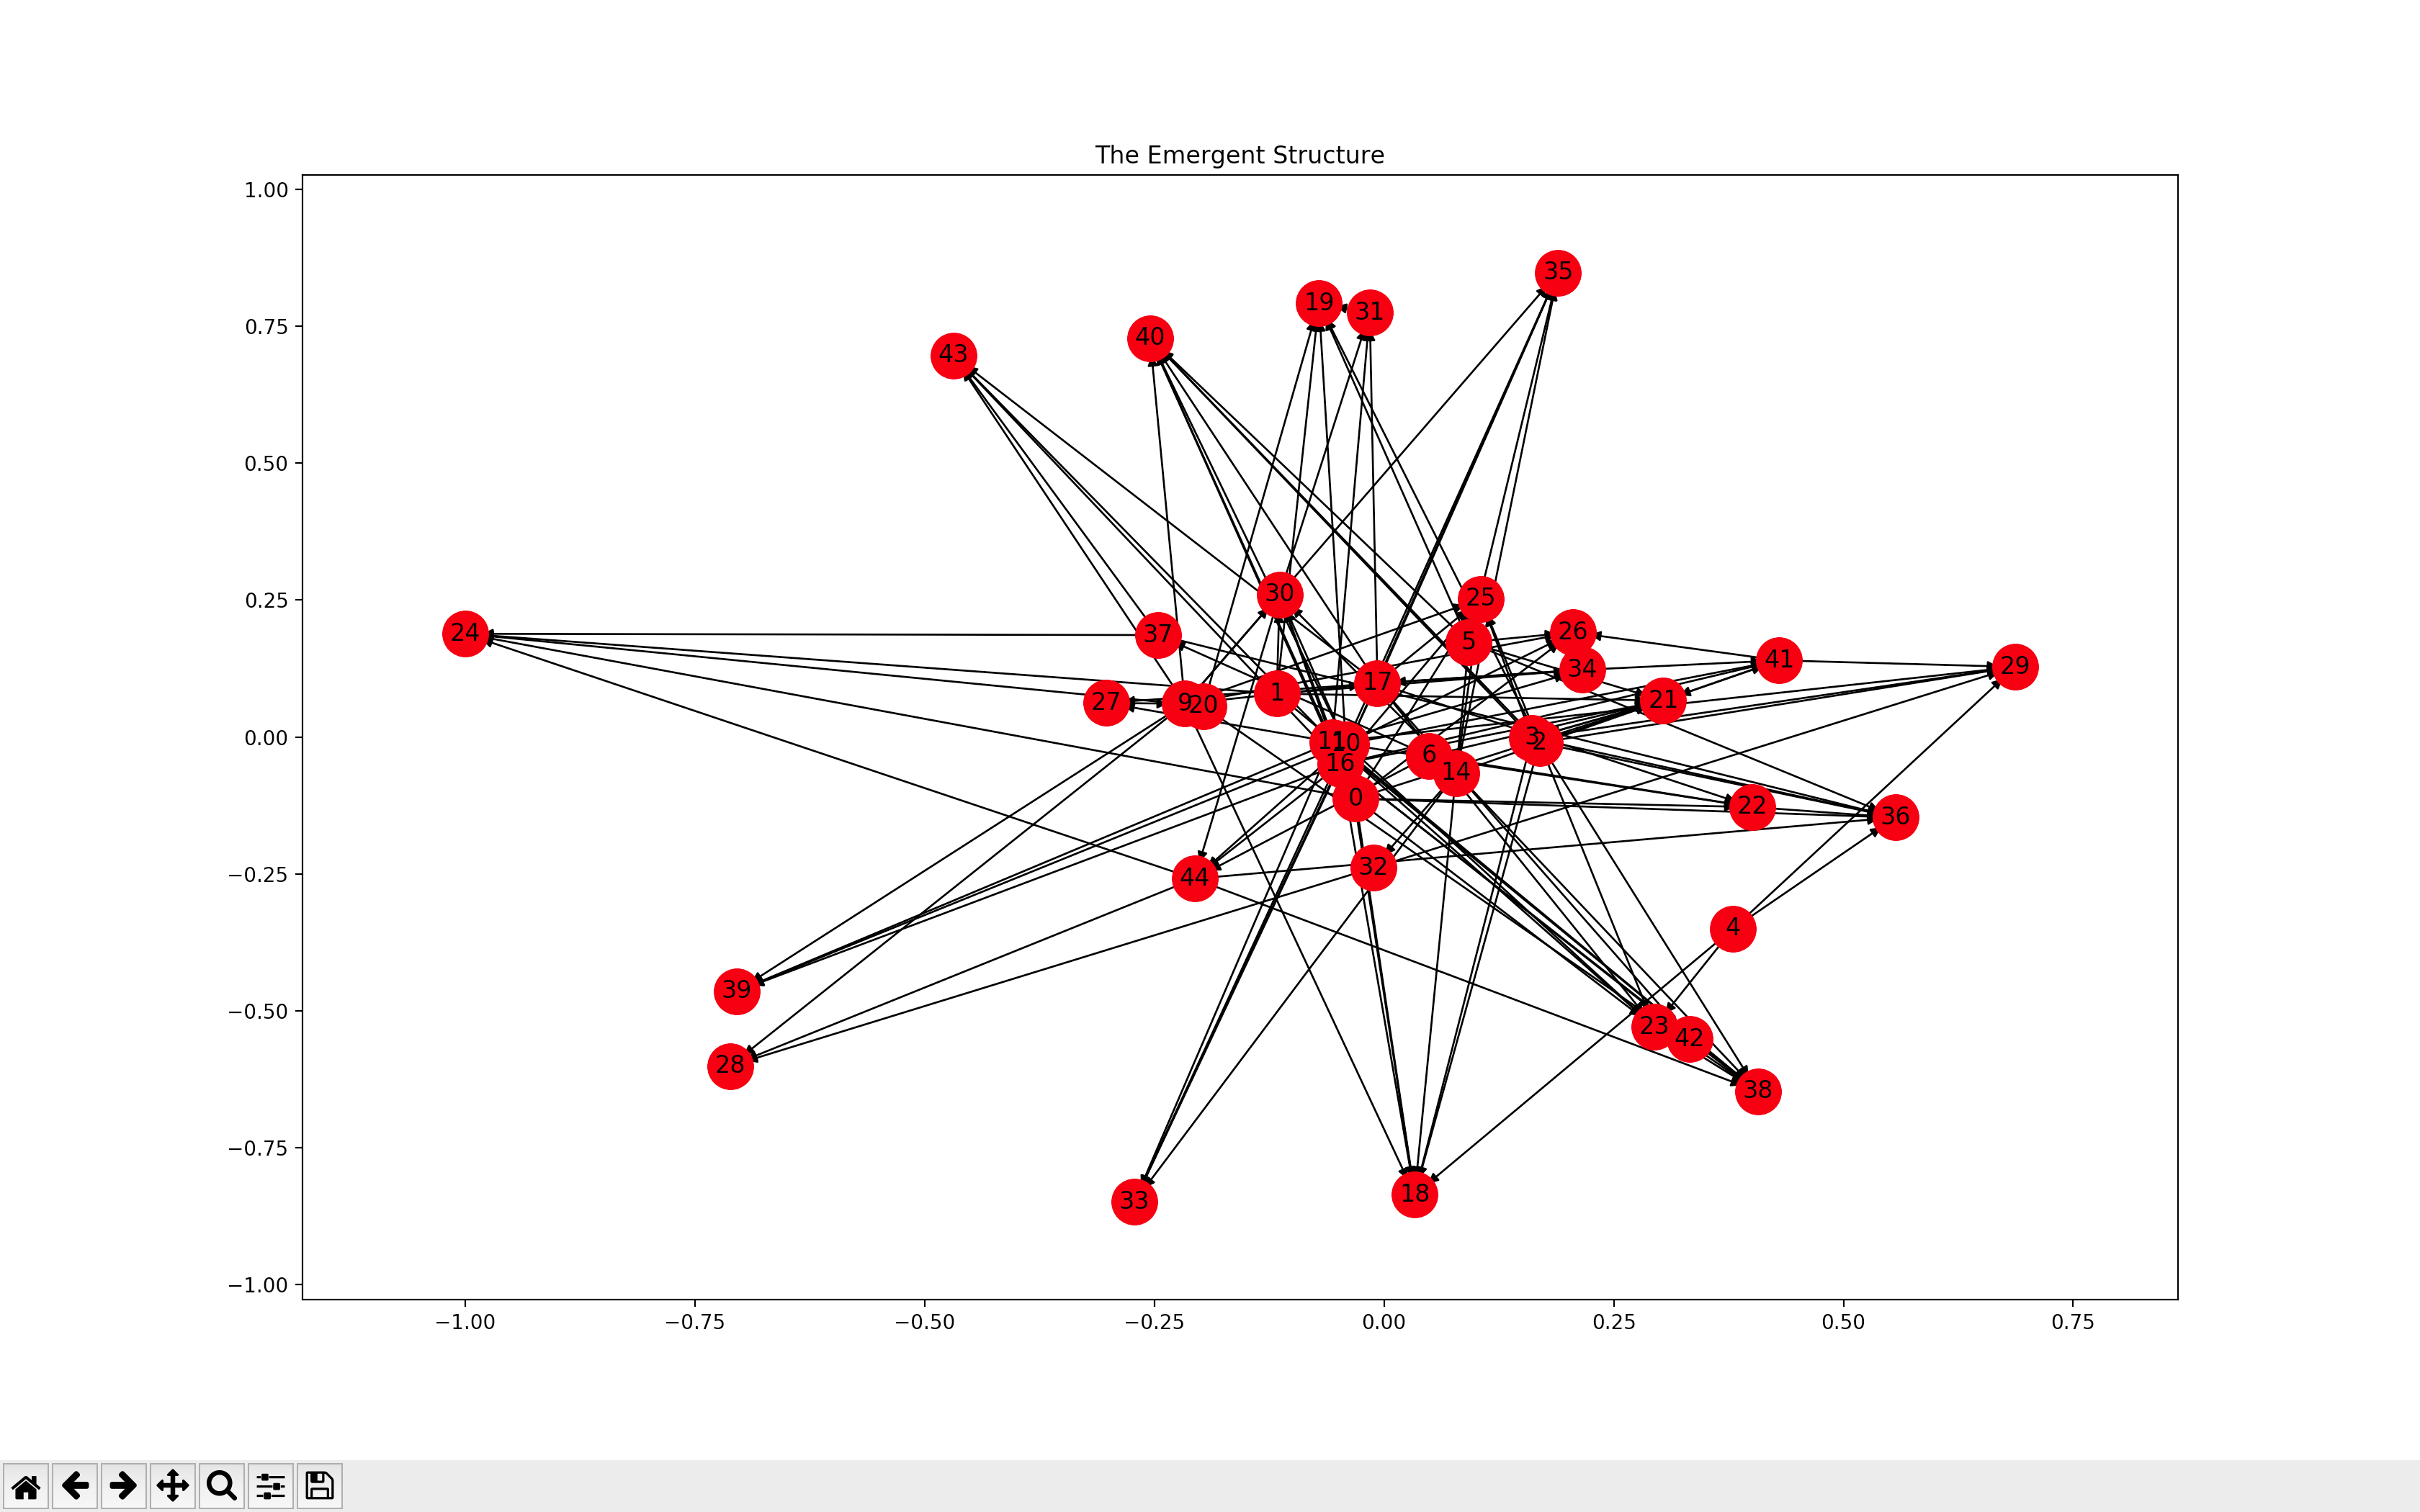
\includegraphics[width=5.8cm]{RNN_Images/8_04} }}%

\subfloat[Threshold=0.03]{{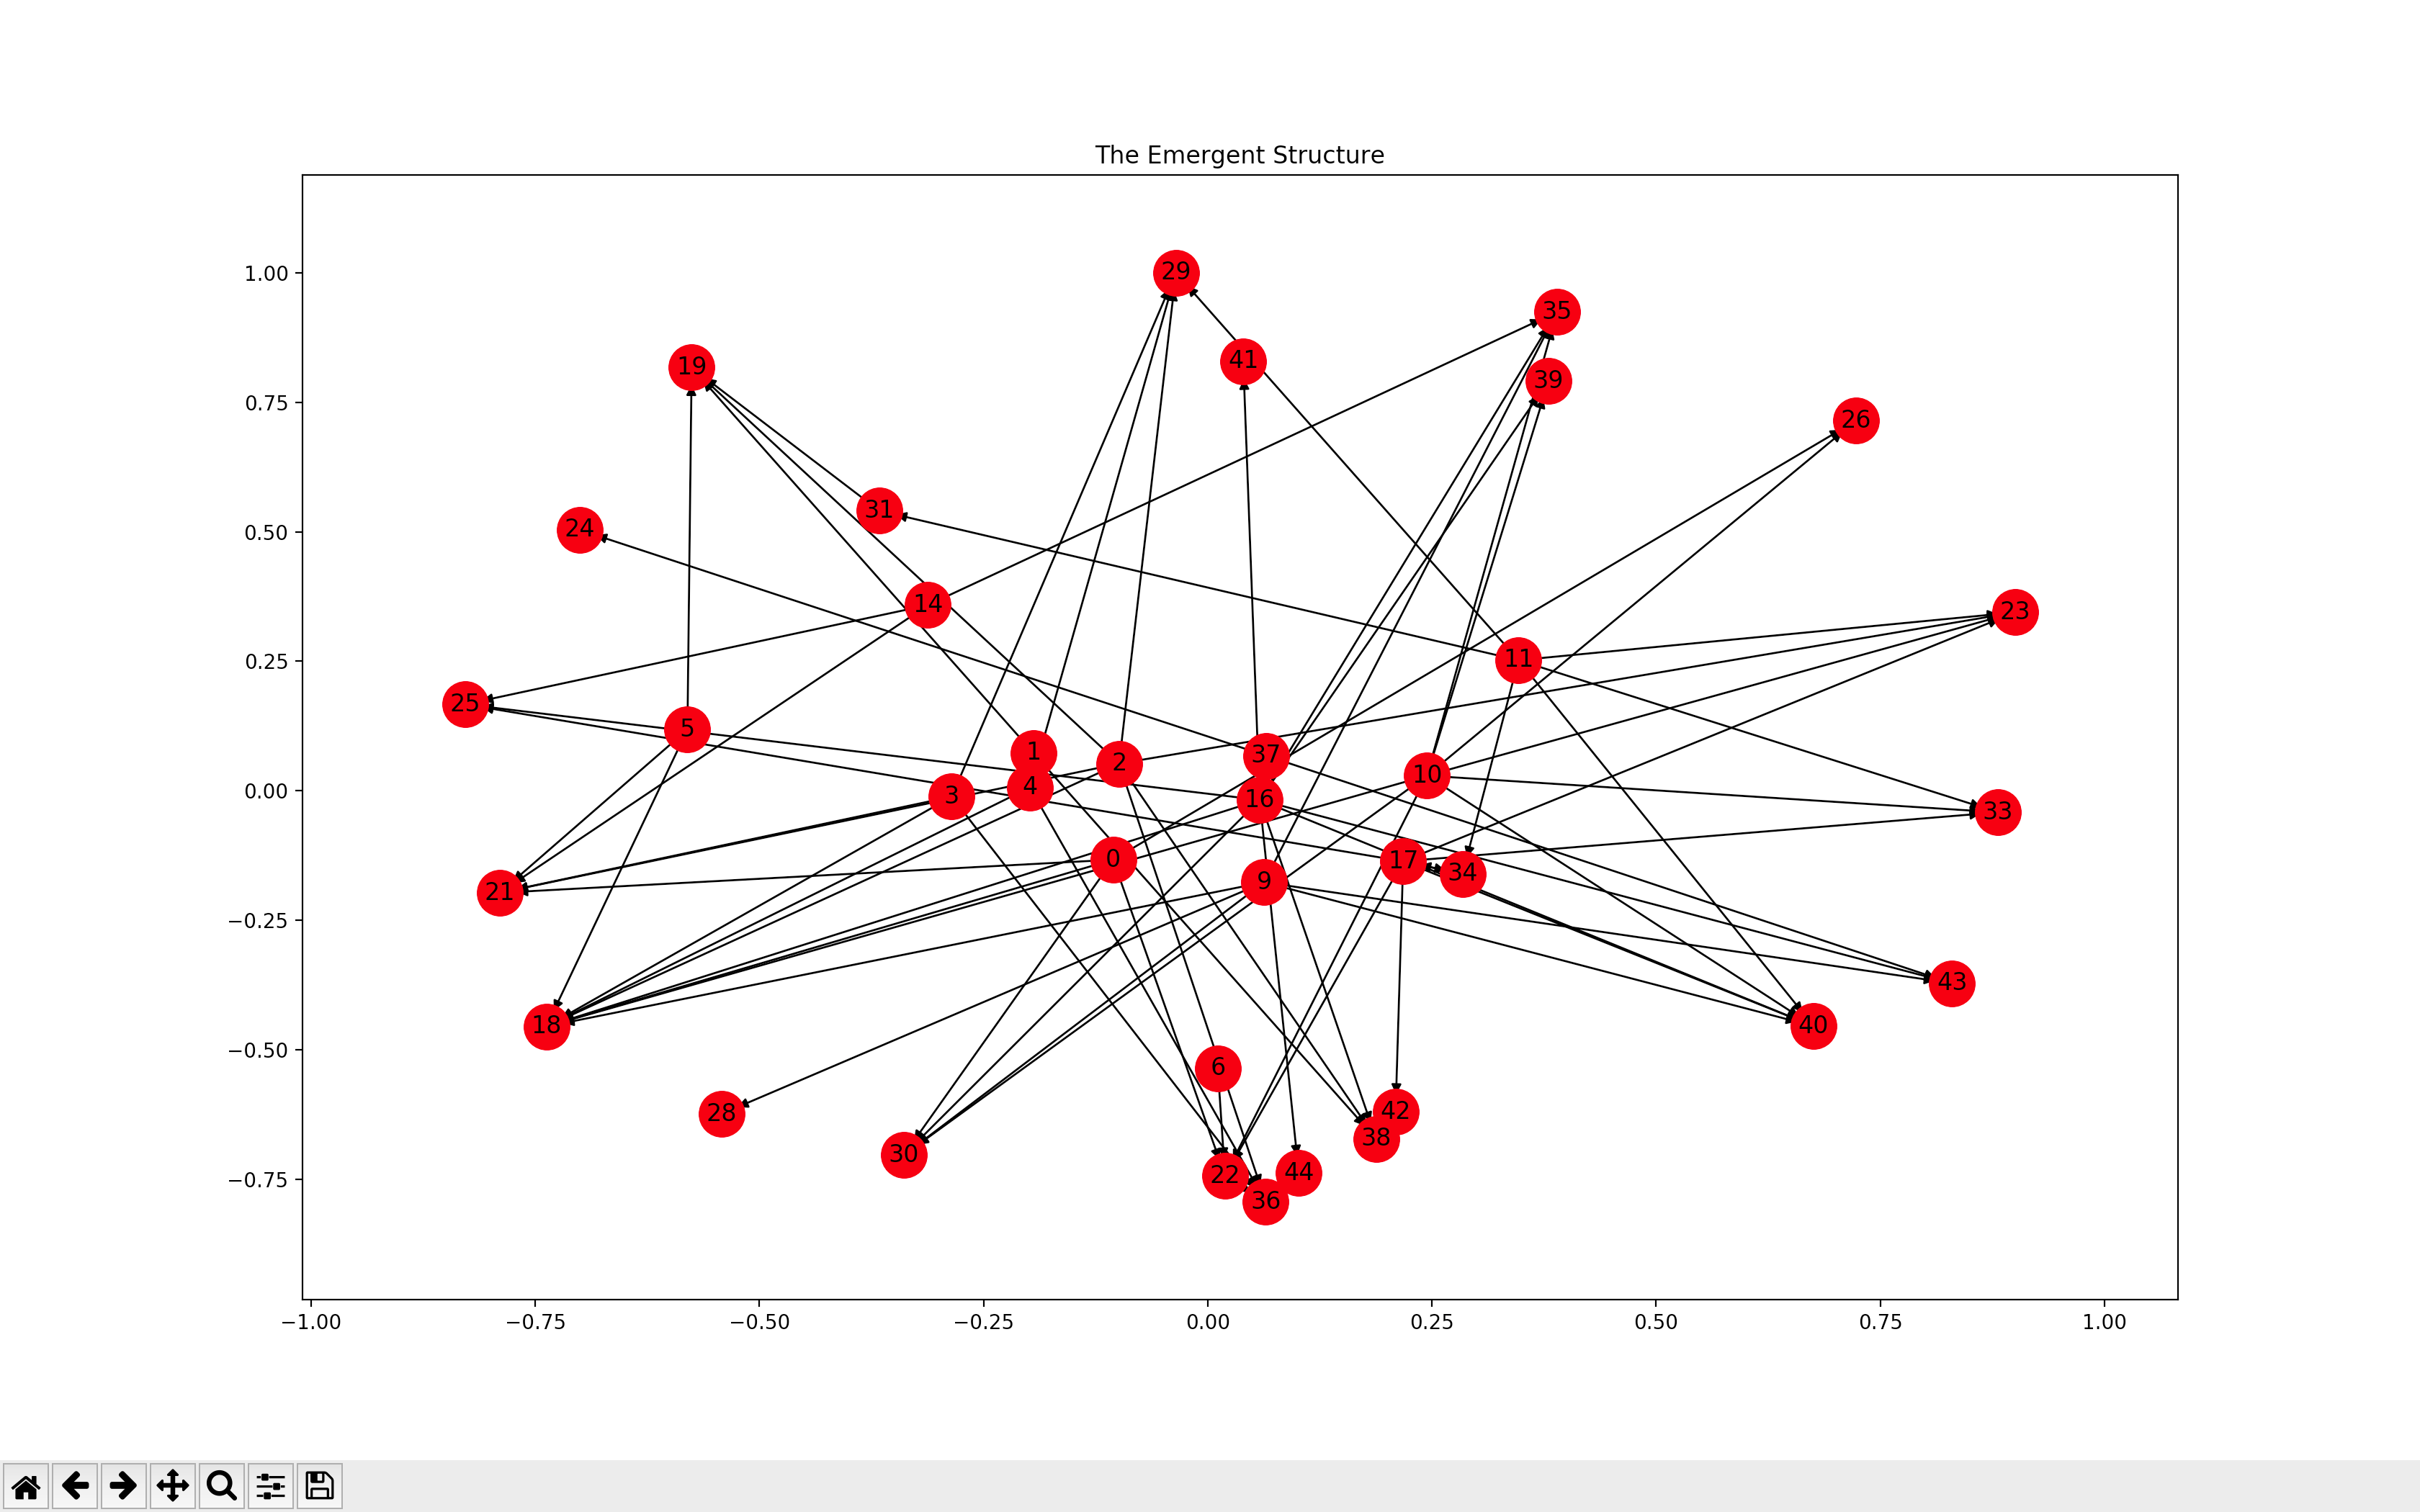
\includegraphics[width=8cm]{RNN_Images/9_03} }}%
\caption{Information Flow Graphs}%
\label{fig:example}%
\end{figure}

 After doing some basic analysis of the graphs, we were not able to find any major patterns. However, we did see a negative correlation between the input degree and output degree. This indicates that some neurons provide information to many neurons and others absorb information from many neurons, but neurons rarely do both. The following plots show this negative correlation.

\begin{figure}[H]
\centering
\noindent
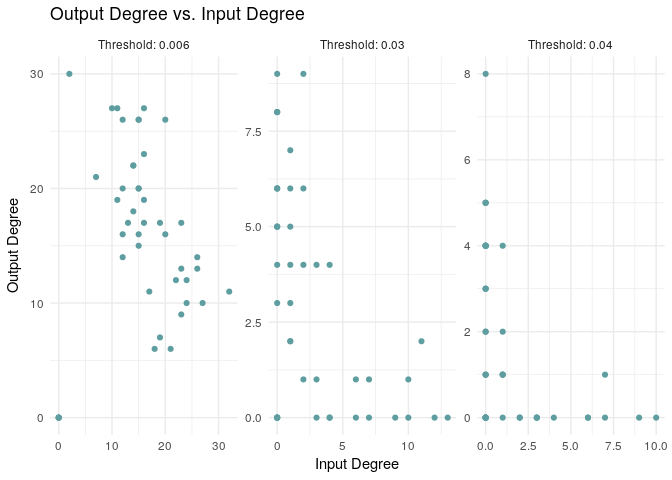
\includegraphics[width=11cm]{RNN_Images/input_1}
\caption{Output Degree vs. Input Degree}%
\label{fig:example}%
\end{figure}

% \begin{figure}[H]
% \centering
% \noindent
% \subfloat[Threshold=0.006]{{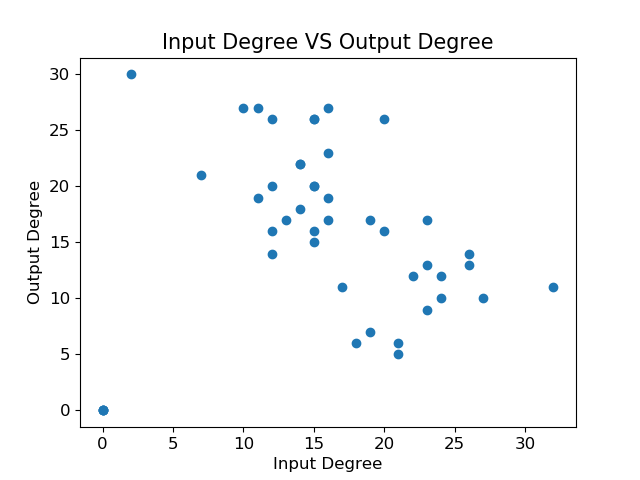
\includegraphics[width=7cm]{RNN_Images/6_006_1} }}%

% \subfloat[Threshold=0.04]{{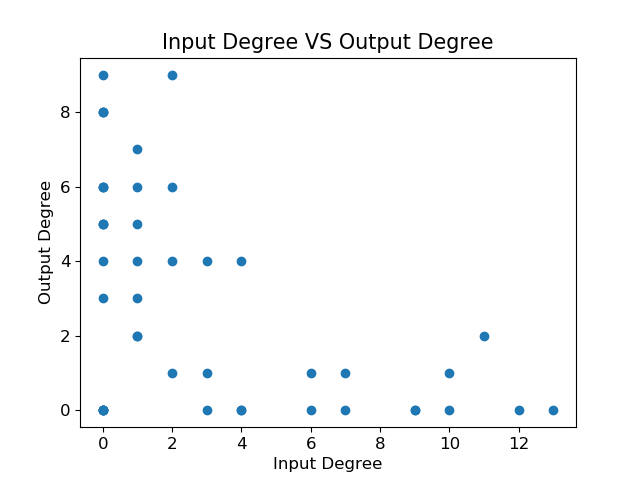
\includegraphics[width=5.8cm]{RNN_Images/4_03_1} }}%
% \subfloat[Threshold=0.03]{{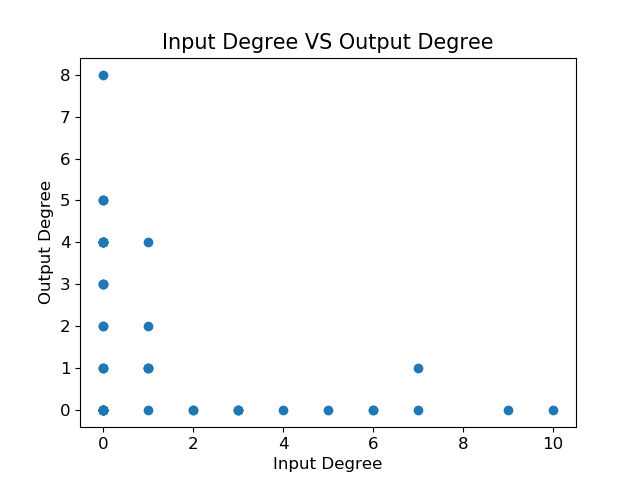
\includegraphics[width=5.8cm]{RNN_Images/5_04_1} }}%
% \caption{Input Degree Vs. Output Degree}%
% \label{fig:example}%
% \end{figure}

Additionally, we have the following degree histograms. These show a lack of any clear pattern in the degrees.

\begin{figure}[H]
\centering
\noindent
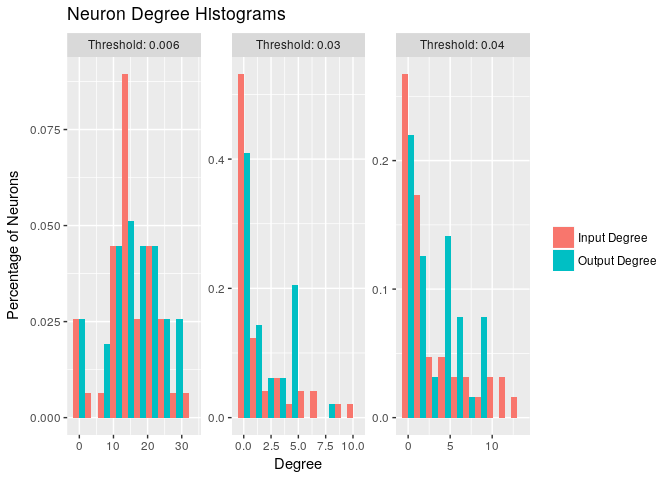
\includegraphics[width=11cm]{RNN_Images/neuron_1}
\caption{Neuron Degree Histograms}%
\label{fig:example}%
\end{figure}

% \begin{figure}[H]
% \centering
% \noindent
% \subfloat[Threshold=0.006]{{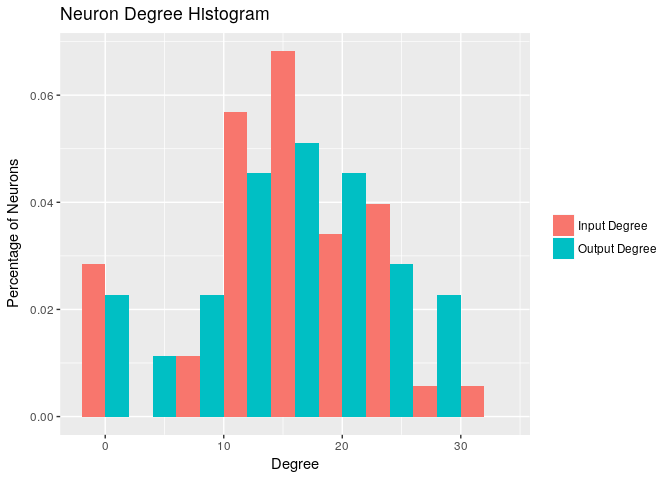
\includegraphics[width=9cm]{RNN_Images/3_CutOff006_2} }}%

% \subfloat[Threshold=0.04]{{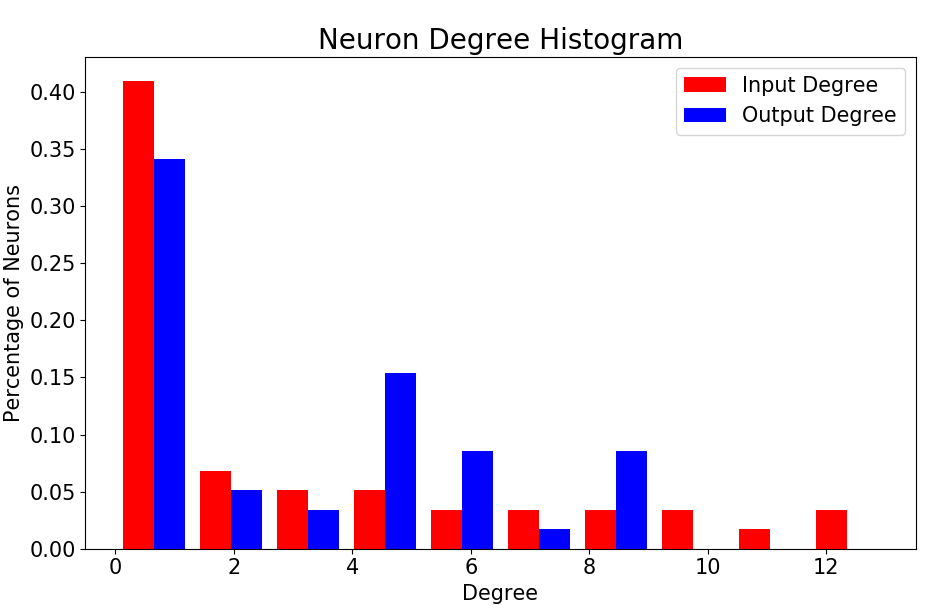
\includegraphics[height=5cm]{RNN_Images/2_CutOff03_1} }}%
% \subfloat[Threshold=0.03]{{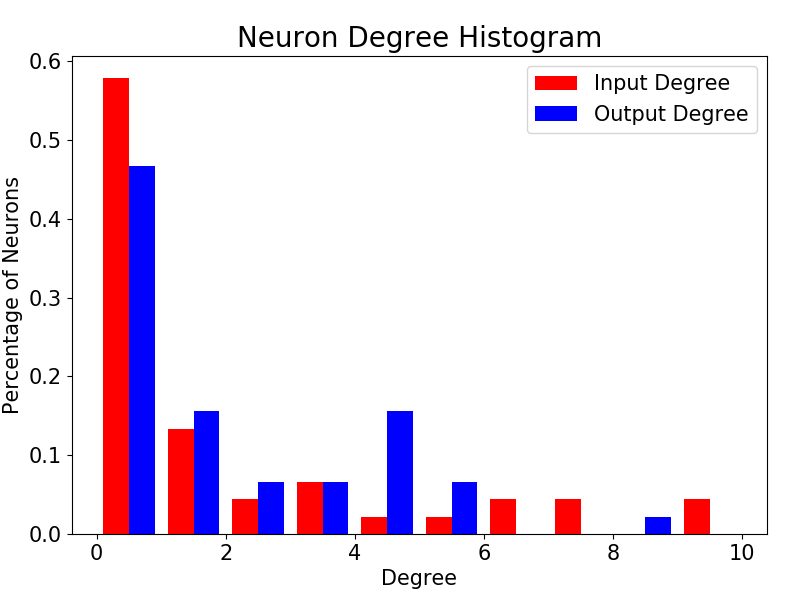
\includegraphics[height=5cm]{RNN_Images/1_CutOff04_1} }}%
% \caption{Neuron Degree Histograms}%
% \label{fig:example}%
% \end{figure}

 \section{The Ranking Algorithm}

 The feature of fully recurrent neural network that separates them from feedforward neural networks is the ability for ever hidden neuron to send information to every other hidden neuron. This removes the natural ordering of the neurons (by layer) that feed forward neural networks have. Therefore, one naturally asks if we can find any ordering to the (hidden) neurons of a fully recurrent neural network, similar to the layers of a feed forward neural network. To do this, we must develop an ordering algorithm to determine an ordering on the neurons from the information flow graph. We say the rank of a neuron is a real number which represents how �far along� the network a certain neuron is. In a feed forward neural network, we expect the rank of the neuron to increase as the layer the neuron is in increases. We define a ranking of the neurons to be a list of ranks of all of the neurons.

 Let $N = \{1, 2, 3, ... n\}$ indicate the set of neurons. Let $r_{i}$ denote the rank of the ith neuron. Let $E_{ij}$ be $1$ if there is an edge from $i$ to $j$ and $0$ otherwise. $E_{ij}$ therefore indicates whether there is a high information flow from $i$ to $j$ or not. Let $I_{i} = \{ j \in N |\ E_{ji} = 1\}$, and $O_{i} = \{ j \in N |\ E_{ij} = 1\}$. $I_{i}$ is the set of neurons that send a high amount of information to $i$, and $O_{i}$ is the set of neurons that receive a high amount of information from $i$. If our network was a feed forward network, we would ideally want the rank of a neuron to be the layer than neuron is in. Alternatively we could represent this desire by saying we ideally want $r_{i} = r_{j} + 1$ if $j$ is in the layer before $i$. The set $I_{i}$  of neurons which send information directly to $i$ should logically be a subset of the neurons in the layer before the layer $i$ is in, so we naturally want $r_{i} = r_{j} + 1$ if $j \in I_{i}$. Similarly, we want $r_{i} = r_{j} - 1$ if $j \in O_{i}$. These desired conditions can now be translated to any neural network (since the notion of ''layer'' is no longer explicit in the conditions). Although it is not always possible to satisfy all these conditions for a recurrent neural network, we can compromise on these requirements with the following condition.
 $$r_{i} = \frac{1}{ | I_{i} | + |O_{i} |}(\sum_{j \in I_{i}} (r_{j} + 1) + \sum_{j \in O_{i}} (r_{j} - 1))$$

 We can define a re-ordering algorithm as taking the rankings of the neurons and recalculating them according to the above equation. Although we got our inspiration from feed forward neural networks, this strategy applies very well to our fully recurrent neural network. We can then define our ranking algorithm as initializing all the ranks to zero and then iteratively applying the re-ranking algorithm until the ranks converge (thus satisfying the desired condition).

 Although we don't a priori have a ranking on our hidden neurons as we would with a feed forward neural network, we do know that logically, our inputs should be ranked before our hidden neurons which should be ranked before our output neurons. Seeing this result in our ranking calculations would provide very strong evidence that our information flow graph and ranking algorithm are accurate. We have the following histograms of the rankings of the inputs, hidden neurons, and outputs (with different information flow cut off points).

\begin{figure}[H]
\centering
\noindent
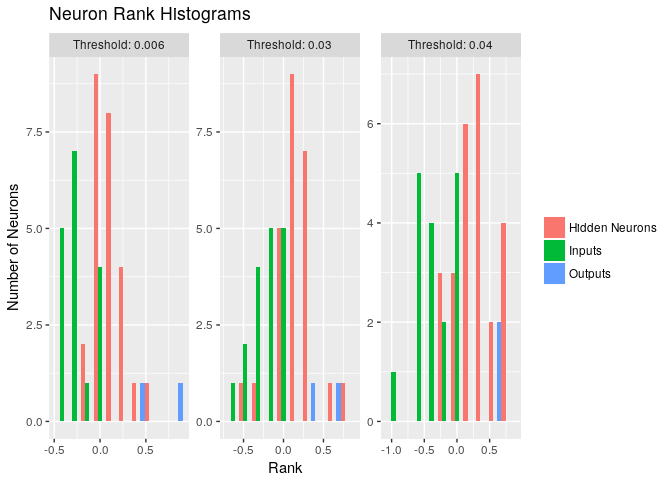
\includegraphics[width=11cm]{RNN_Images/rank_1}%
\caption{Neuron Ranking Histograms}%
\label{fig:example}%
\end{figure}

% \begin{figure}[H]
% \centering

% \subfloat[Threshold=0.006]{{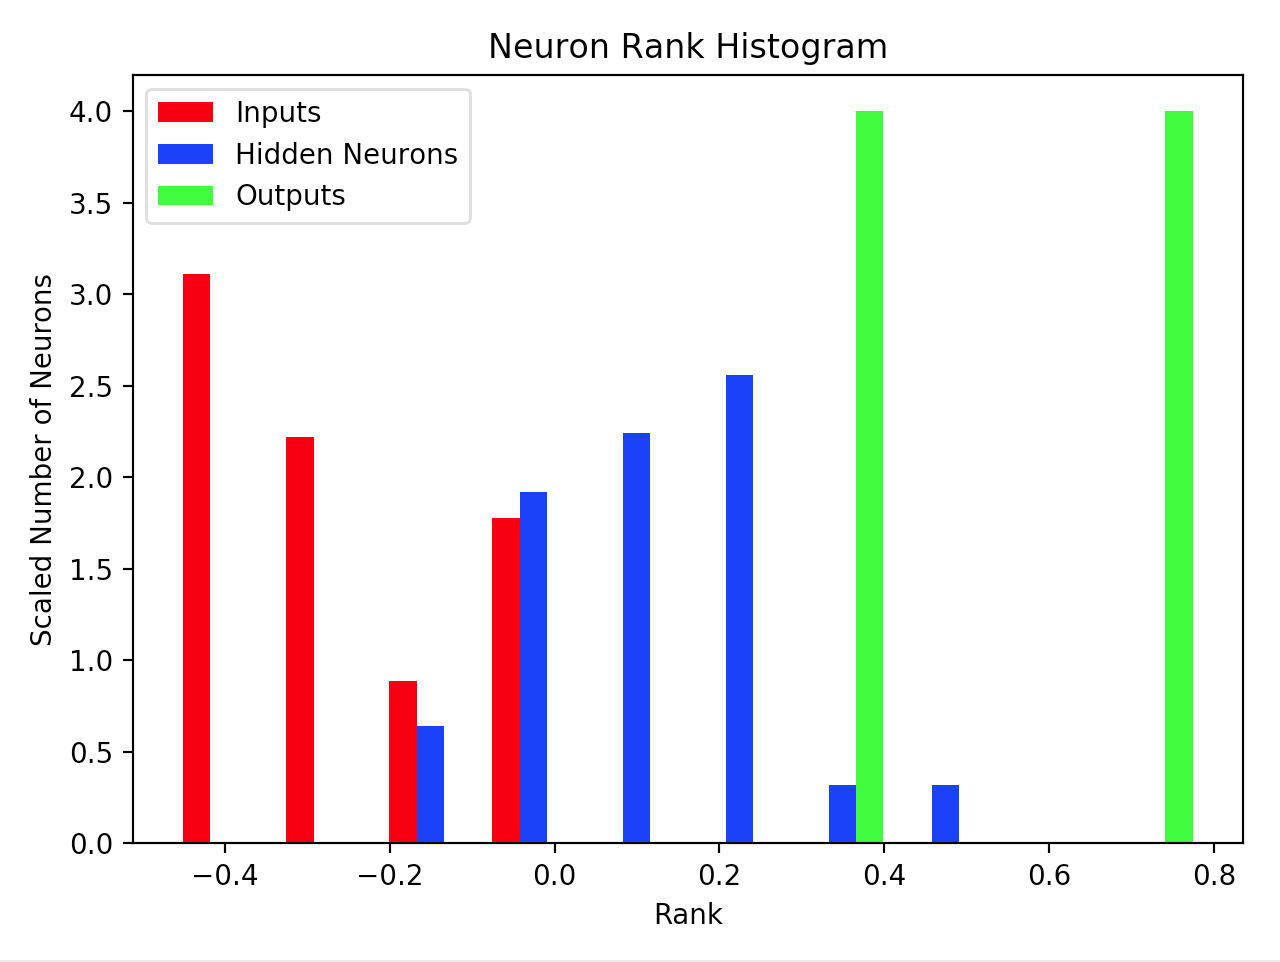
\includegraphics[width=7cm]{RNN_Images/22} }}%

% \noindent
% \subfloat[Threshold=0.04]{{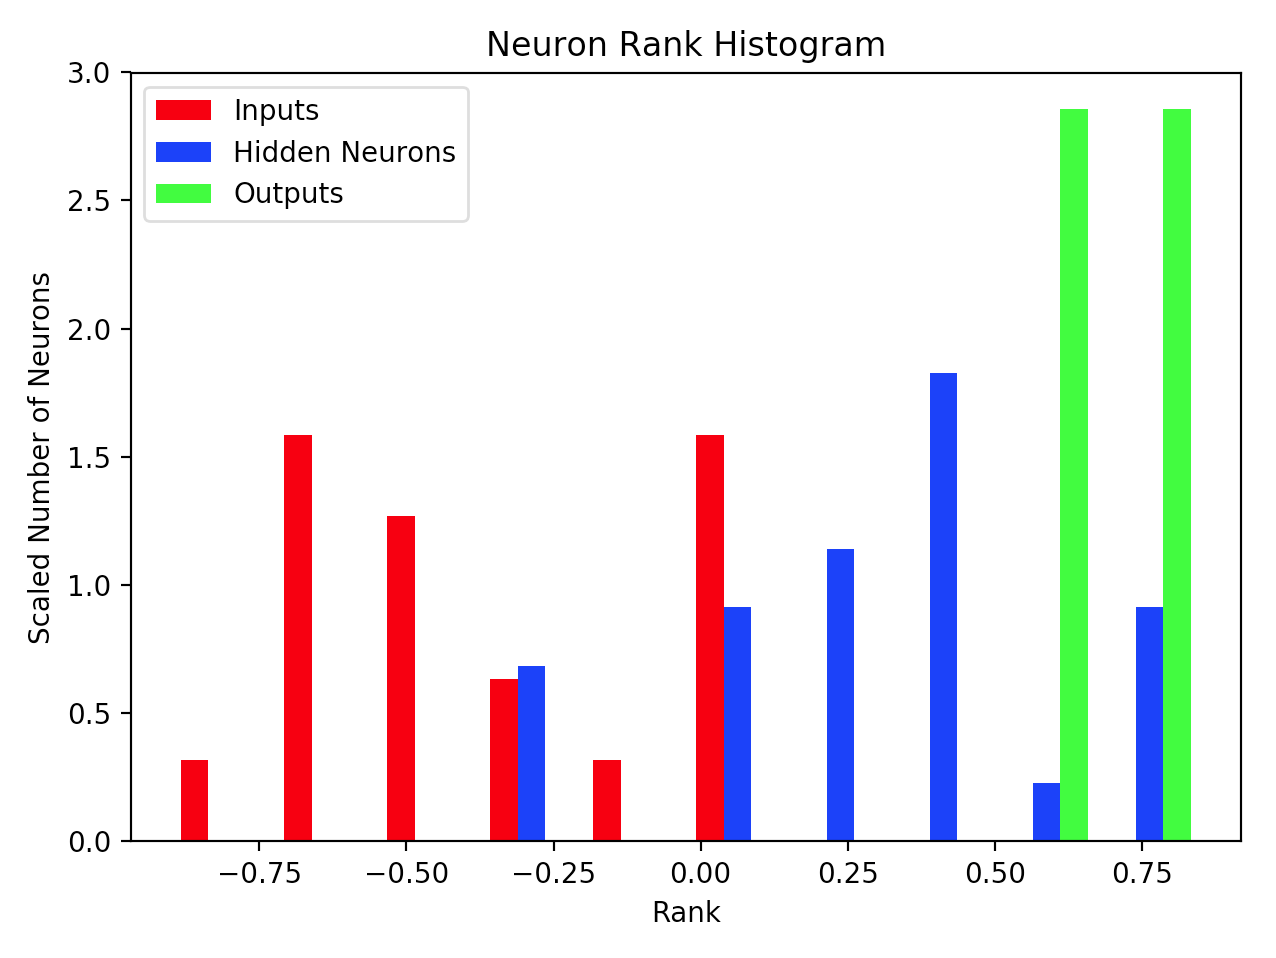
\includegraphics[width=5.8cm]{RNN_Images/23} }}%
% \subfloat[Threshold=0.03]{{\includegraphics[width=5.8cm]{RNN_Images/241} }}%
% \caption{Neuron Ranking Histograms}%
% \label{fig:example}%
% \end{figure}

  Note, the algorithms not always exactly ranking the inputs before the hidden neurons before the outputs is not always incorrect. For example, if we had the toy network with the connections Input $\rightarrow$ A $\rightarrow$ B $\rightarrow$ C $\rightarrow$ D $\rightarrow$ E $\rightarrow$ Output, and Input $\rightarrow$ F $\rightarrow$ Output, one could reasonably rank A before the input because it takes 5 steps to go from A to the Output, yet only 2 steps to go from the input to the output. This is only a toy example, however, it shows that a bit of ''error'' in ranking the inputs, outputs, and hidden neurons is not necessarily a bad thing (although not generally fitting that ordering certainly would be bad sign). Aside from this, we do not see much interesting structure (or patterns) in the rankings. However, that is likely a result of our network having too few neurons to find statistically significant patterns. In a network with a large amount of neurons, the ranking could be used to reveal ''layer'' like structures. These structures would be formed out of groups of neurons doing computations in parallel with similar sources and sinks of information, and could be revealed by statistically significant spikes in the ranking histogram. Since we do not have enough neurons to effectively do this analysis, we applied a separate analysis to try to find these structures in which we looked at the similarity between sources and sinks of information between pairs of neurons. However, the results were inconclusive.

  \section{Input and Output Mutual Information During Testing}

  Another thing we can test to try to probe the natural structure of the network is analyzing the mutual information of each neuron with the input layer and ground truth outputs during training. If we get a negative correlation between the mutual information with the input and mutual information with the output, this would show the neurons ''forgetting'' information about the inputs as they better fit the outputs. This would provide evidence for the information bottleneck principle applying to fully recurrent neural networks during testing (although this is a somewhat different application of the information bottleneck principle than what was researched in ''Opening the black box of Deep Neural Networks via Information''). However, this is not what we see.

\begin{figure}[H]
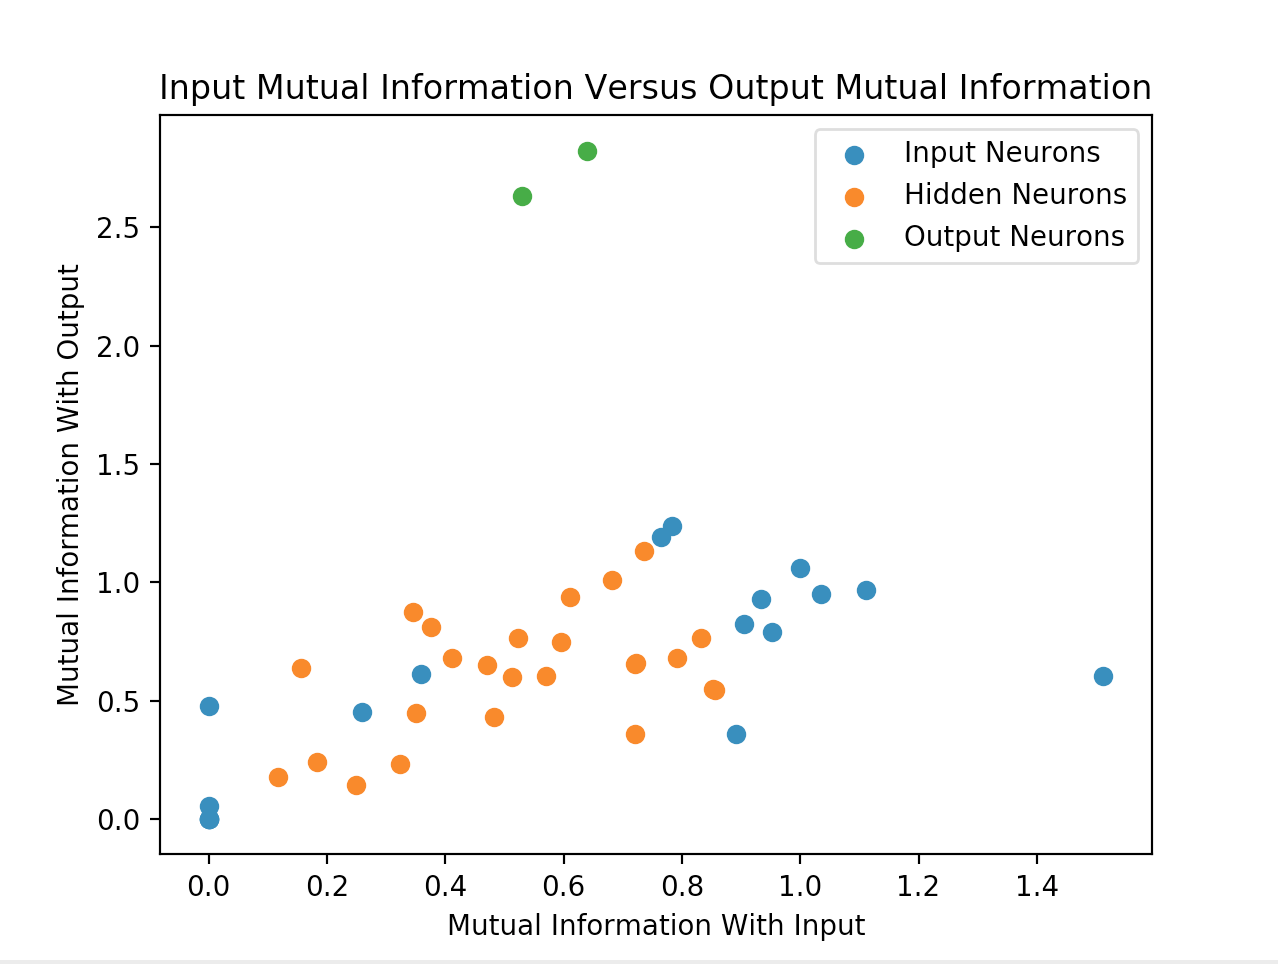
\includegraphics[width=8cm]{RNN_Images/11}
\centering
\caption{Input vs Output Mutual Information: All Neurons}%
\end{figure}

We see that the output neurons both have high mutual information with the ground truth output, as expected. These two neurons do not reveal any interesting results, so we can remove them from the plot and get the following.

\begin{figure}[H]
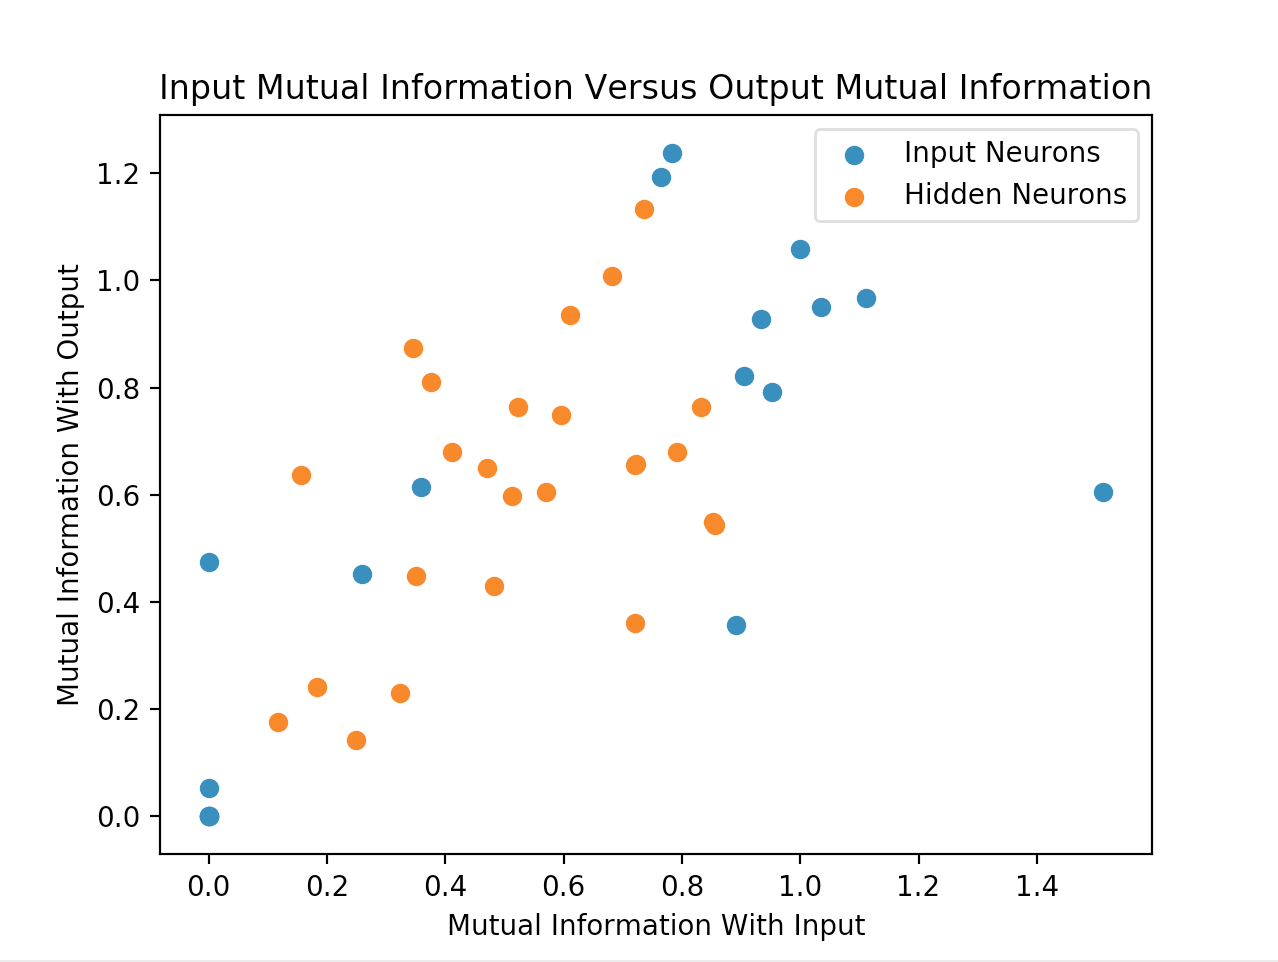
\includegraphics[width=8cm]{RNN_Images/10}
\centering
\caption{Input vs Output Mutual Information: No Outputs}%
\end{figure}

 There clearly appears to be a positive correlation between the mutual information with the inputs and the mutual information with the outputs. One might think that this could be caused by some neurons simply having more information than others. However, if we divide by the total amount of information (the entropy) of each neuron, we get the following plot.

\begin{figure}[H]
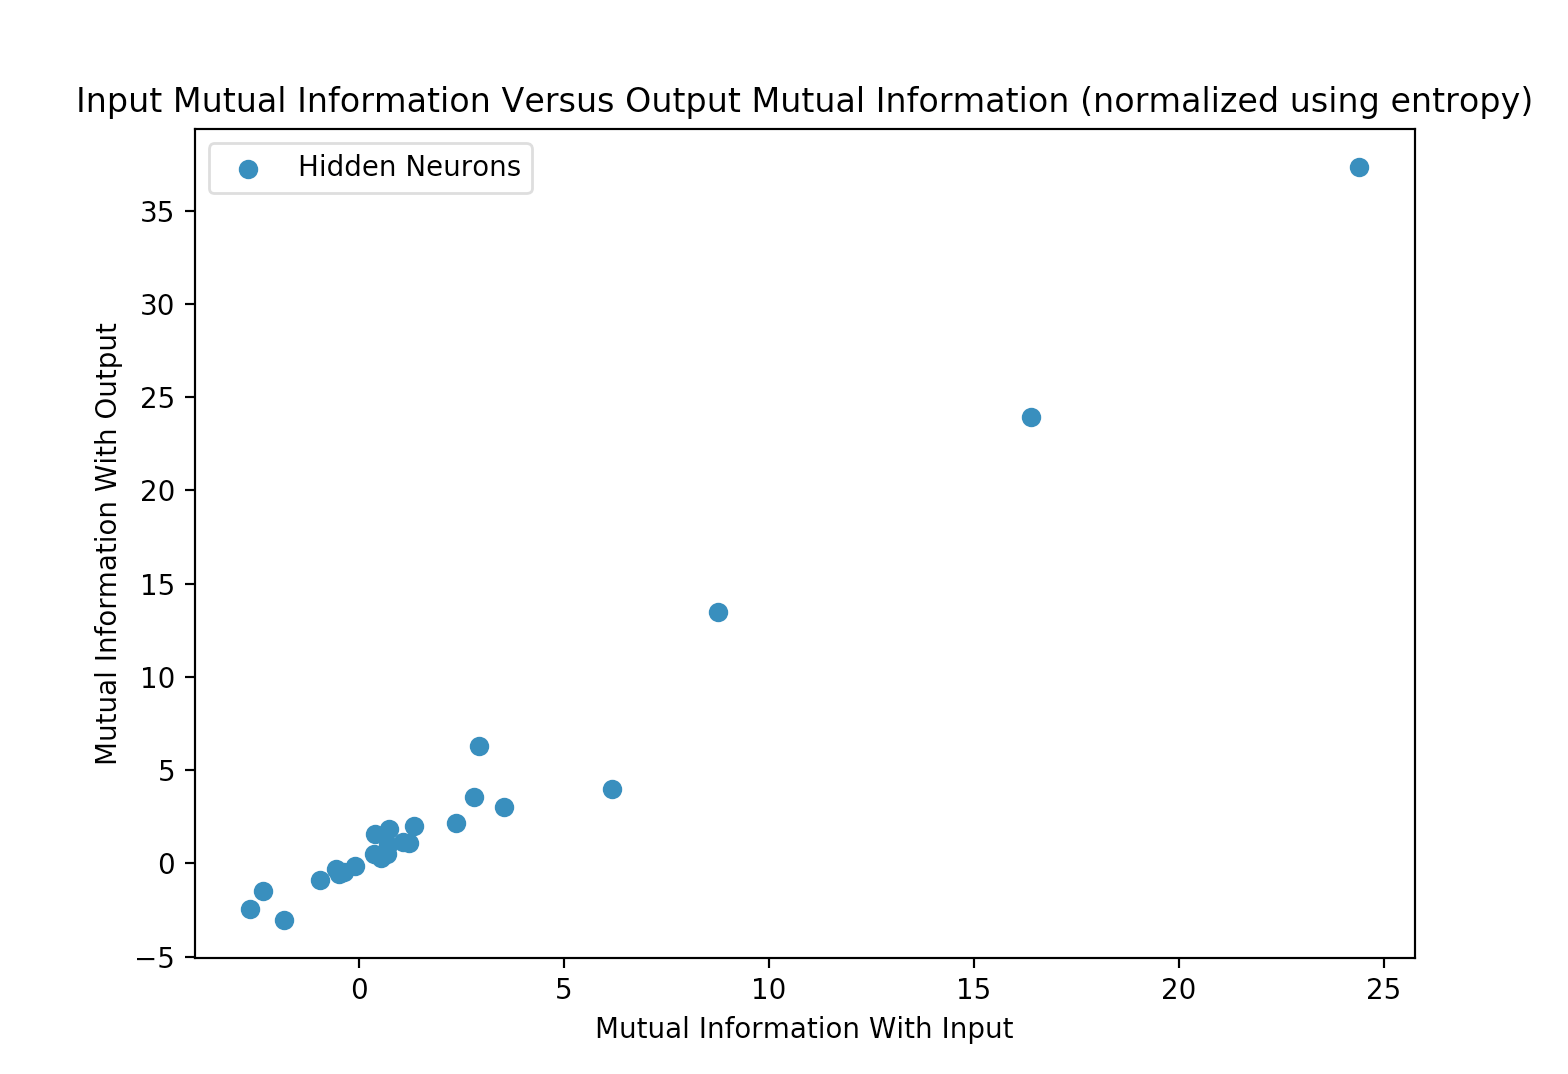
\includegraphics[width=8cm]{RNN_Images/12}
\centering
\caption{Input vs Output Mutual Information: Entropy Normalization}%
\end{figure}

 This plot has an even higher positive correlation, so we can dismiss that possibility as the reason for the positive correlation. Note, we should not read too much into this increased positive correlation when dividing by the entropy, since this ''positive correlation'' is also what we would expect if the entropy was just a widely varying random variable. In my opinion, the most likely explanation for the positive correlation between the mutual information with the input and the mutual information with the output is just that some neurons are more important than others. The more important neurons then have a higher mutual information with both the input and the output. A very simple example where this could occur is if we are trying to replicate some function with multiple underlying processes. If some neurons are dedicated to each process, and not all the processes are equally important, this naturally results in widely varying neuron importance, in even an ideal network. It is very reasonable to expect this to be the case for our task (weather prediction).

  \section{Input and Output Mutual Information During Training}

All plots in this section will have one data point per 10 epochs. We will therefore refer to adjacent epochs as epochs differing by 10. Also, all plots are scaled to maximize at 1.

In addition to looking at the mutual information of the neurons with the inputs and ground truth outputs during testing (as in the last section), we can see how these values change during training. If we do this for each neuron in the hidden layer individually, the plot is very chaotic and hard to follow. It is much nicer to look at the mutual information between the entire hidden layer and the inputs and ground truth outputs. This results in the following plot. We use a line plot instead of a scatter plot in order to help convey the order of the data points in terms of what epoch they are in. Specifically, values at adjacent epochs are connected by lines and the first epoch is  the leftmost point.

\begin{figure}[H]
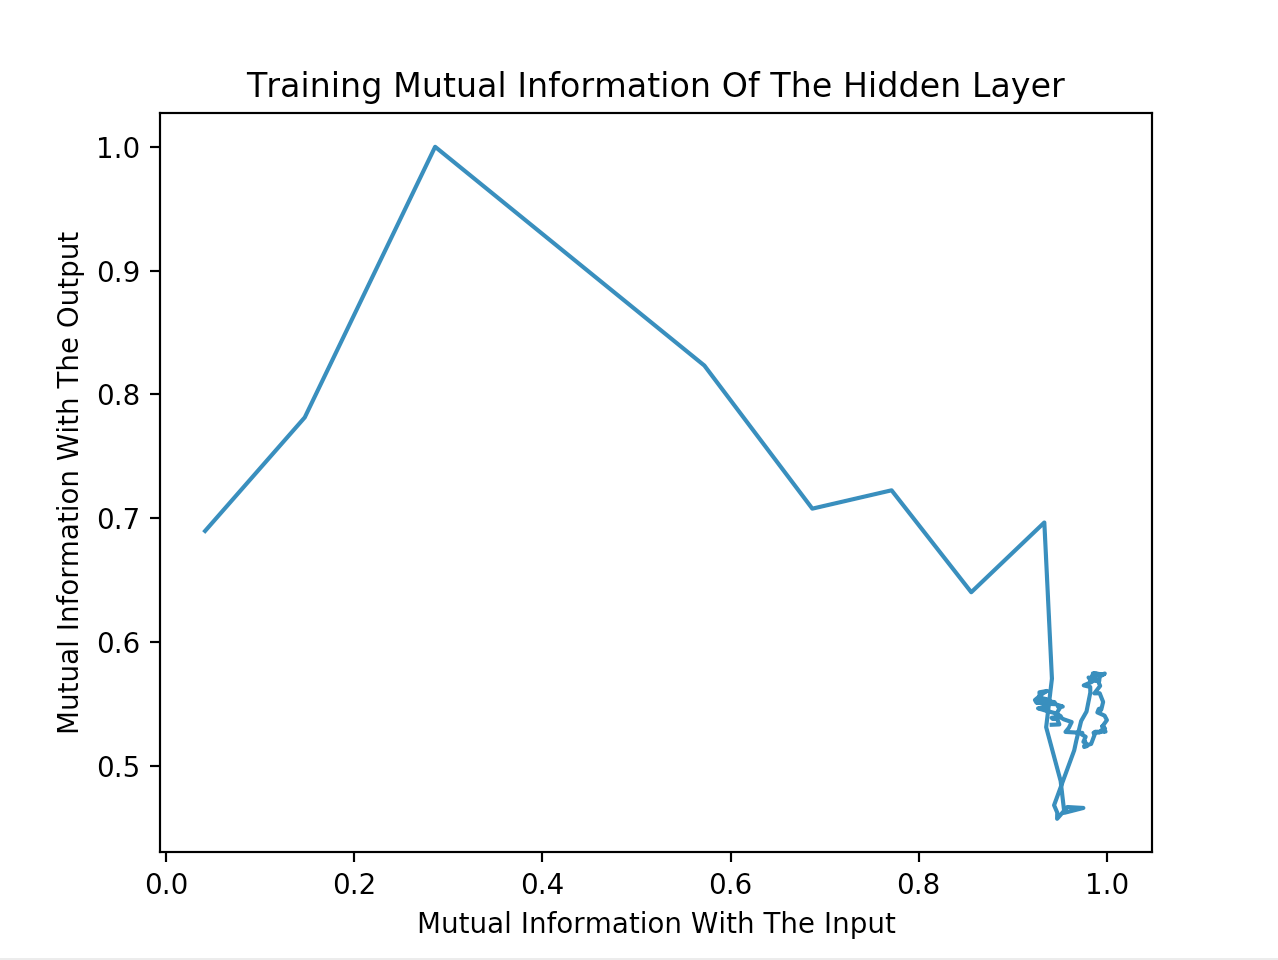
\includegraphics[width=8cm]{RNN_Images/13}
\centering
\caption{Hidden Layer Mutual Information During Training}%
\end{figure}


 If the information bottleneck principle applied to our fully recurrent neural network, we would expect the mutual information with the input to first increase and then begin to decrease. We would also expect this (decreasing) to happen with the mutual information between the hidden neurons and the ground truth output, but to a much smaller extent. Instead, we only see the mutual information with the input increase (not decrease). We also see the mutual information with the output increase, then decrease, then increase again, then decrease again, and then increase again. The learning does seem to be split into two phases, like how learning for feed forward neural networks can be split into two phases according to ''Opening the black box of Deep Neural Networks via Information'' , however, the phases are very different from feed forward neural networks. These phases are not likely to be purely noise due to them happening continuously over many many epochs, however, they may only be applicable to our network for our task. We were not able to come up with any theoretical justification to the phases of learning we see. Looking at the mutual information of the outputs (both the individual neurons and the layer as a whole) with the inputs and ground truth outputs we get the following plots.


 \begin{figure}[H]
\centering

\noindent
\subfloat[The Full Layer]{{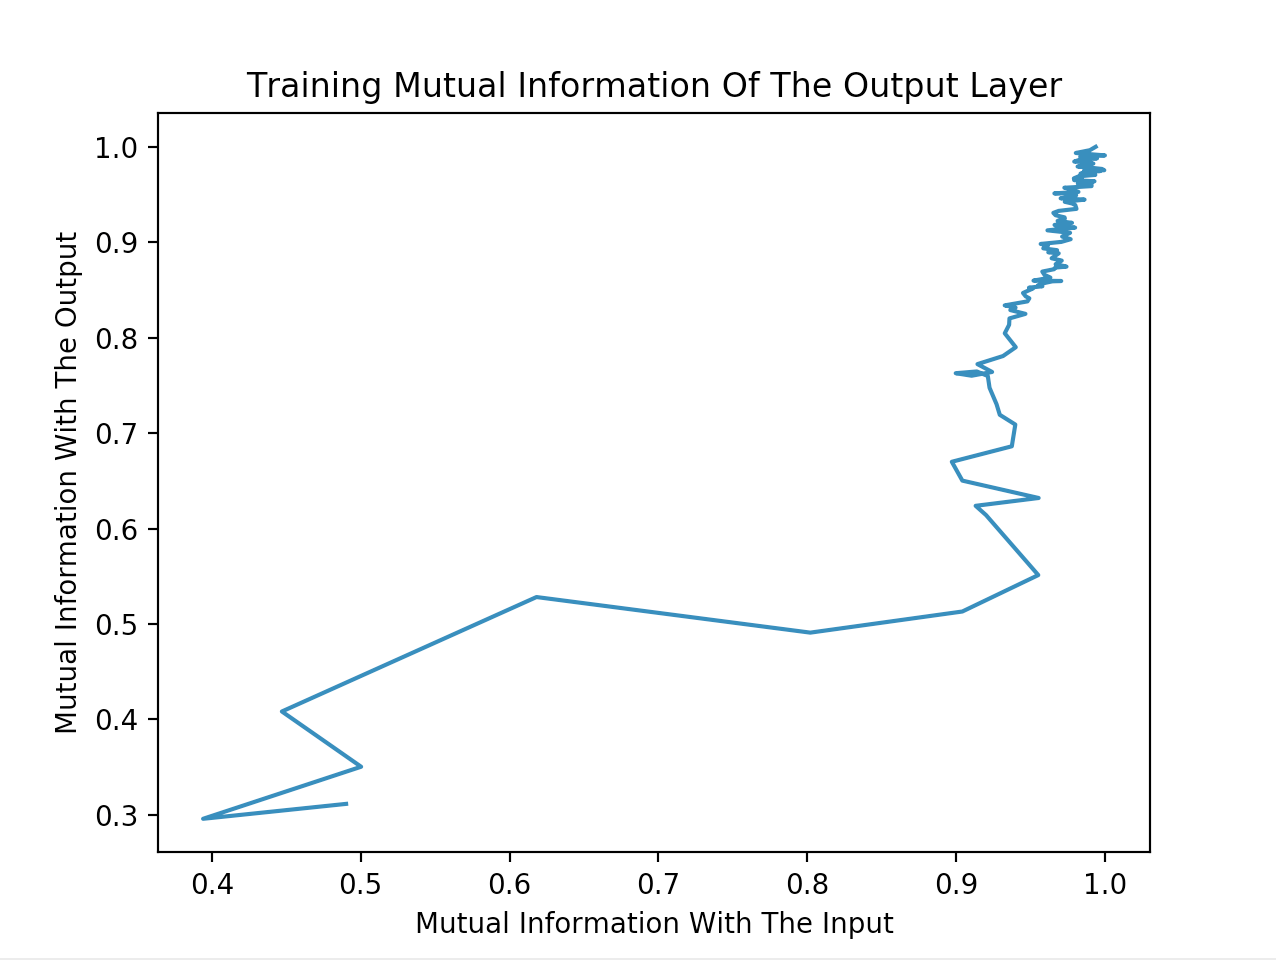
\includegraphics[width=5.8cm]{RNN_Images/14} }}%
\subfloat[Individual Neurons]{{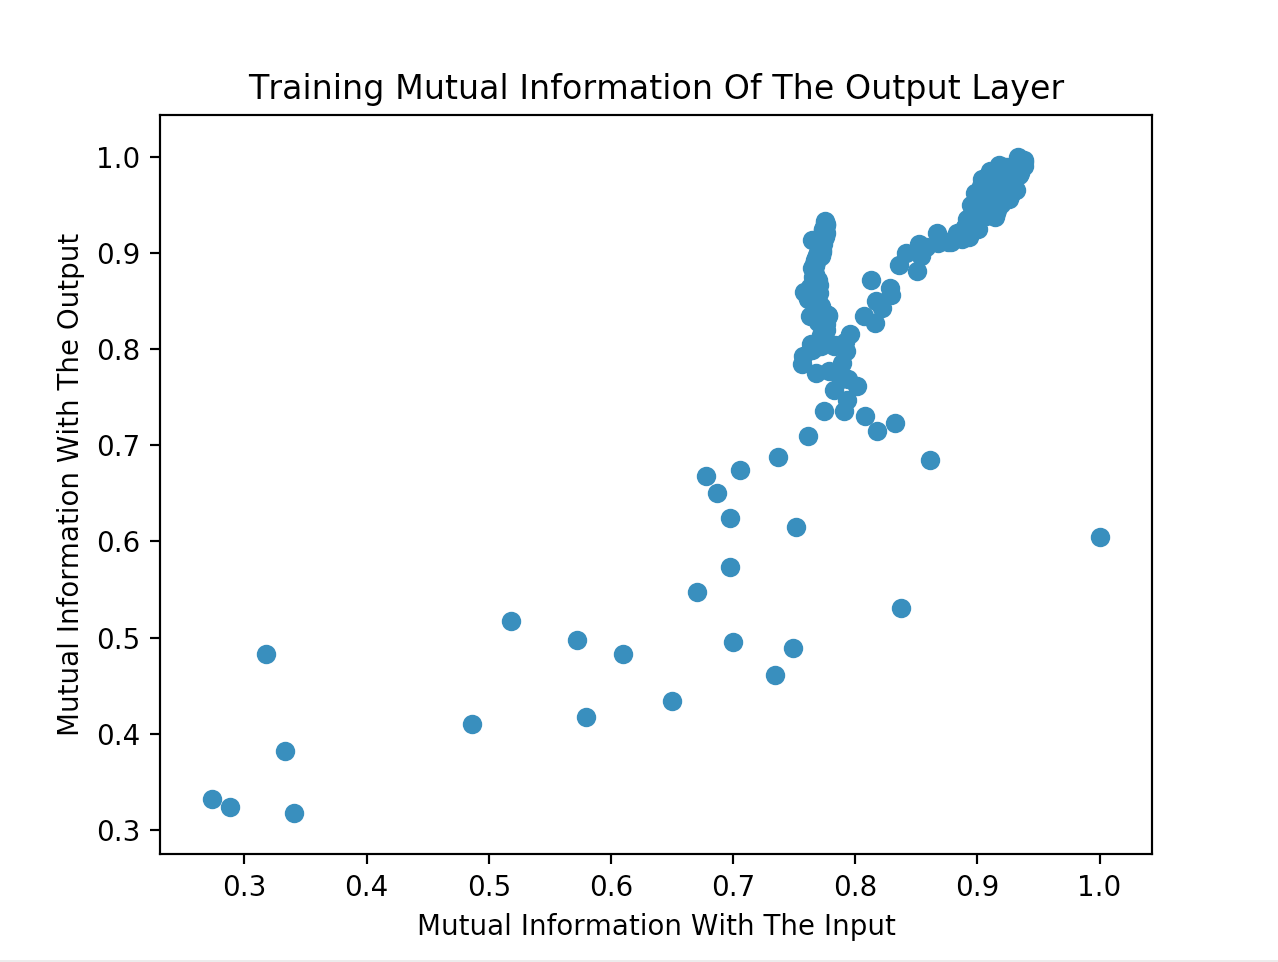
\includegraphics[width=5.8cm]{RNN_Images/15} }}%
\caption{Output Layer Mutual Information During Training}%
\label{fig:example}%
\end{figure}

 Here we also do not see any indication of the information bottleneck principle applying. In fact, unlike with the hidden neurons, the mutual information with the ground truth outputs never decreases. The network just learns to use the information about the ground truth outputs stored within the hidden layer more efficiently (as that stored information decreases). It is possible that the mutual information between the hidden neurons and the ground truth output decreases while the output layer learns to use that information more efficiently, and then begins to increase again once the information is being used as efficiently as feasible (and thus more information about the ground truth output must begin to be stored in the hidden layer). However, that is purely a hypothesis, and we have no empirical evidence of this idea. We created the following plot of the error and the mutual information between the hidden layer and the ground truth output to try to give more hints to understanding this phenomena.

\begin{figure}[H]
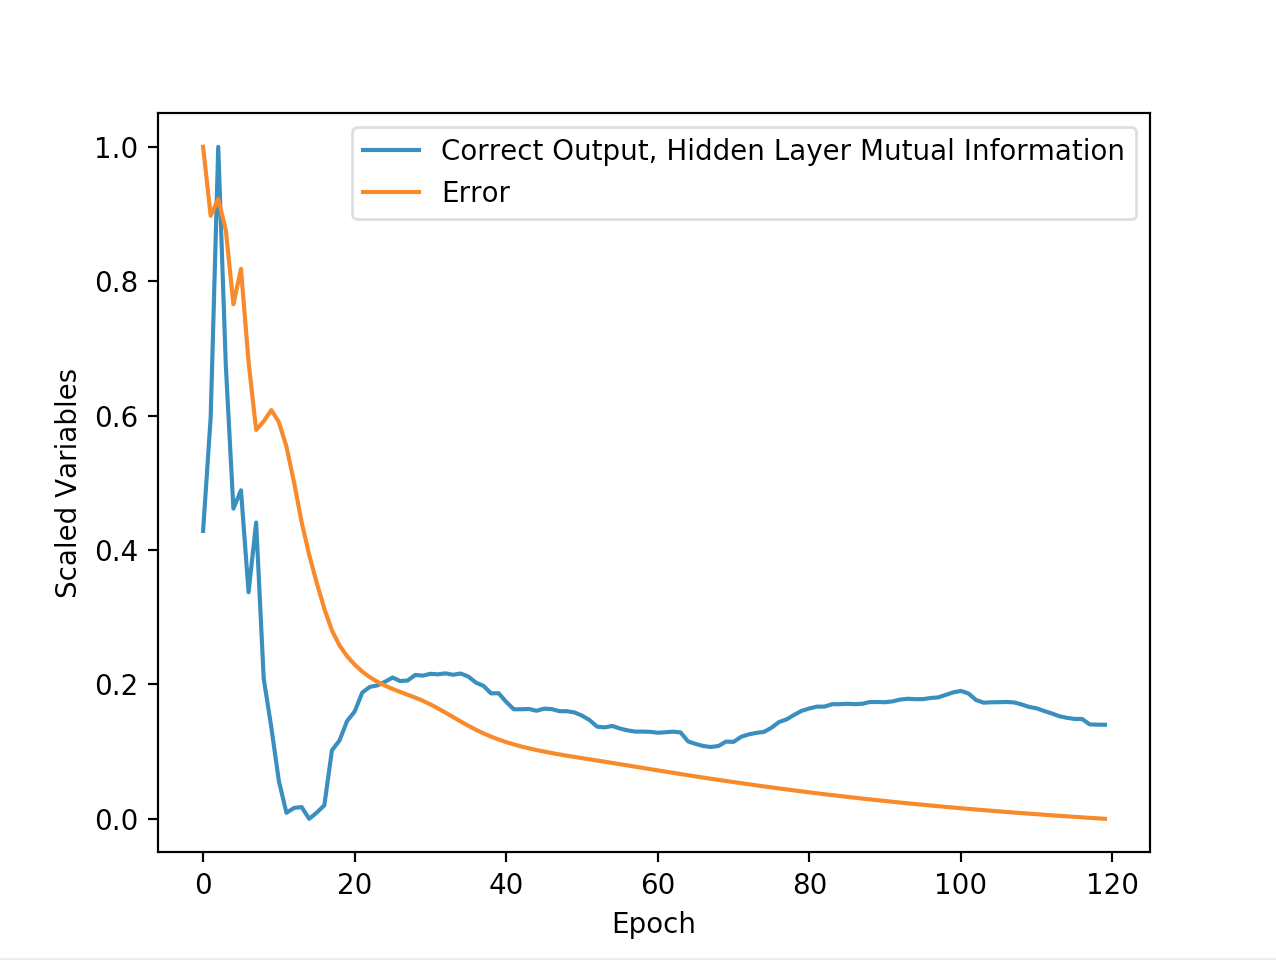
\includegraphics[width=7cm]{RNN_Images/20}
\centering
\caption{Hidden Layer and Ground Truth Output Mutual Information During Training}%
\end{figure}

 The majority of the error decreasing appears to be happening as the mutual information with the ground truth output is decreasing (which is the opposite of what one would naturally expect); However, we have no evidence that this is not just a coincidence. Applying our analyses to other fully recurrent neural networks in the future could potentially help see if this is meaningful.

 \section{An Analysis of Learning Indicators}

 In ''Information Theory for Analyzing Neural Networks'' it was shown that the mutual information of the neurons with the input and ground truth output is a useful learning indicator. This usefulness is primarily a result of the mutual information increasing before the error starts significantly decreasing. As stated in ''Information Theory for Analyzing Neural Networks'', ''This, I believe, is very useful, especially for classifiers, as it can take several epochs before we see any significant drop in the error rate''. We test if we can replicate this result for a fully recurrent neural network, and test for other learning indicators. Mutual information between the output layer and the ground truth output almost perfectly mimics the (negative of) the error (as one would naturally expect) as in the following plot.

\begin{figure}[H]
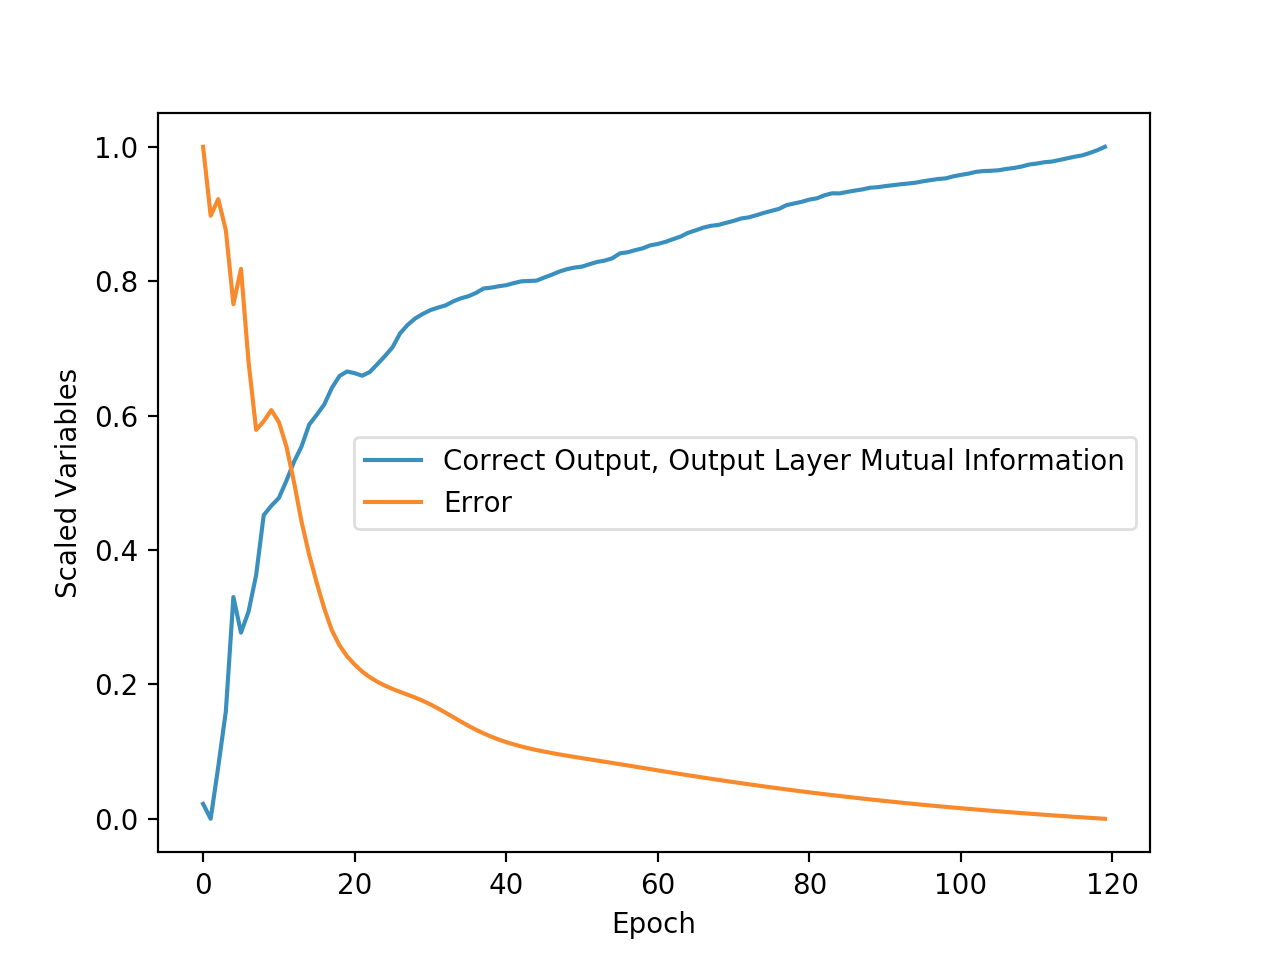
\includegraphics[width=8cm]{RNN_Images/25}
\centering
\caption{Output Layer and Ground Truth Output Mutual Information During Training}%
\end{figure}

 However, this is not a useful indicator because it does not provide any information which is not provided by the error. The mutual information between the hidden layer and the ground truth output has somewhat odd behavior during training (as shown in the previous section) and is therefore not necessarily a useful learning indicator. The mutual information of the hidden or output layer with the input, however, seems to be a very effective learning indicator.

\begin{figure}[H]
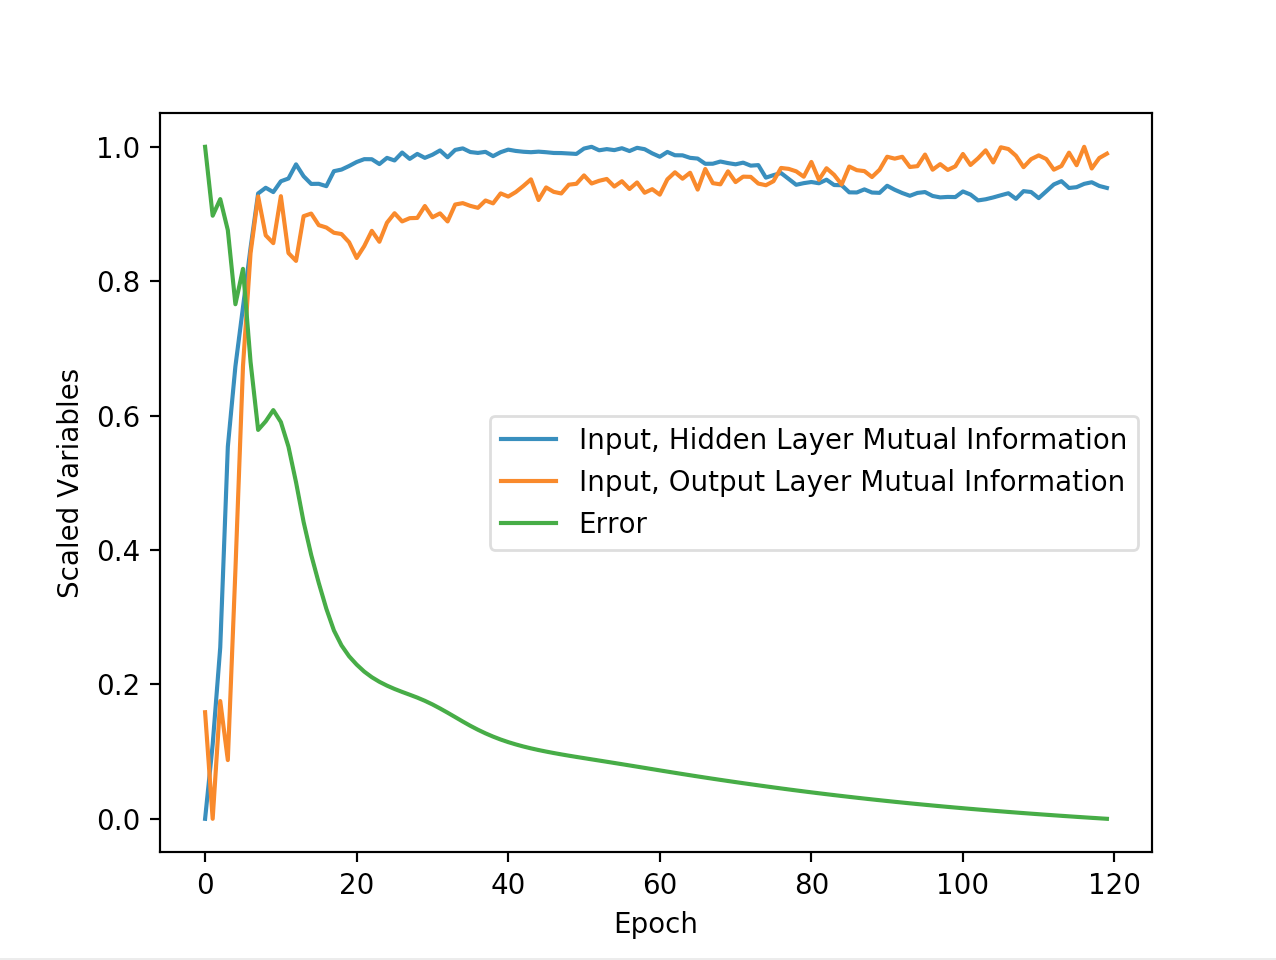
\includegraphics[width=7cm]{RNN_Images/21}
\centering
\caption{Hidden Layer and Input Mutual Information During Training}%
\end{figure}

The above plot clearly shows the mutual information with the input increasing far faster than the error decreases. We also note that the mutual information between the input and the output is almost identical to the mutual information between the input and the hidden neurons. Therefore, clearly, they make equally good learning indicators. In addition to these mutual information measurements we found one other very effective learning indicator, TSE complexity. To calculate the TSE complexity in polynomial time, we approximated averages over all subsets of size k by averages over some randomly choose subset of the set of all subsets of size k. To ensure our approximation was valid, we tried varying the number of subsets chosen, and the results were altered only insignificantly. Not only was the TSE complexity a good learning indicator, but it also almost identically behaved like the mutual information with the input. The bellow plot shows this behavior.

\begin{figure}[H]
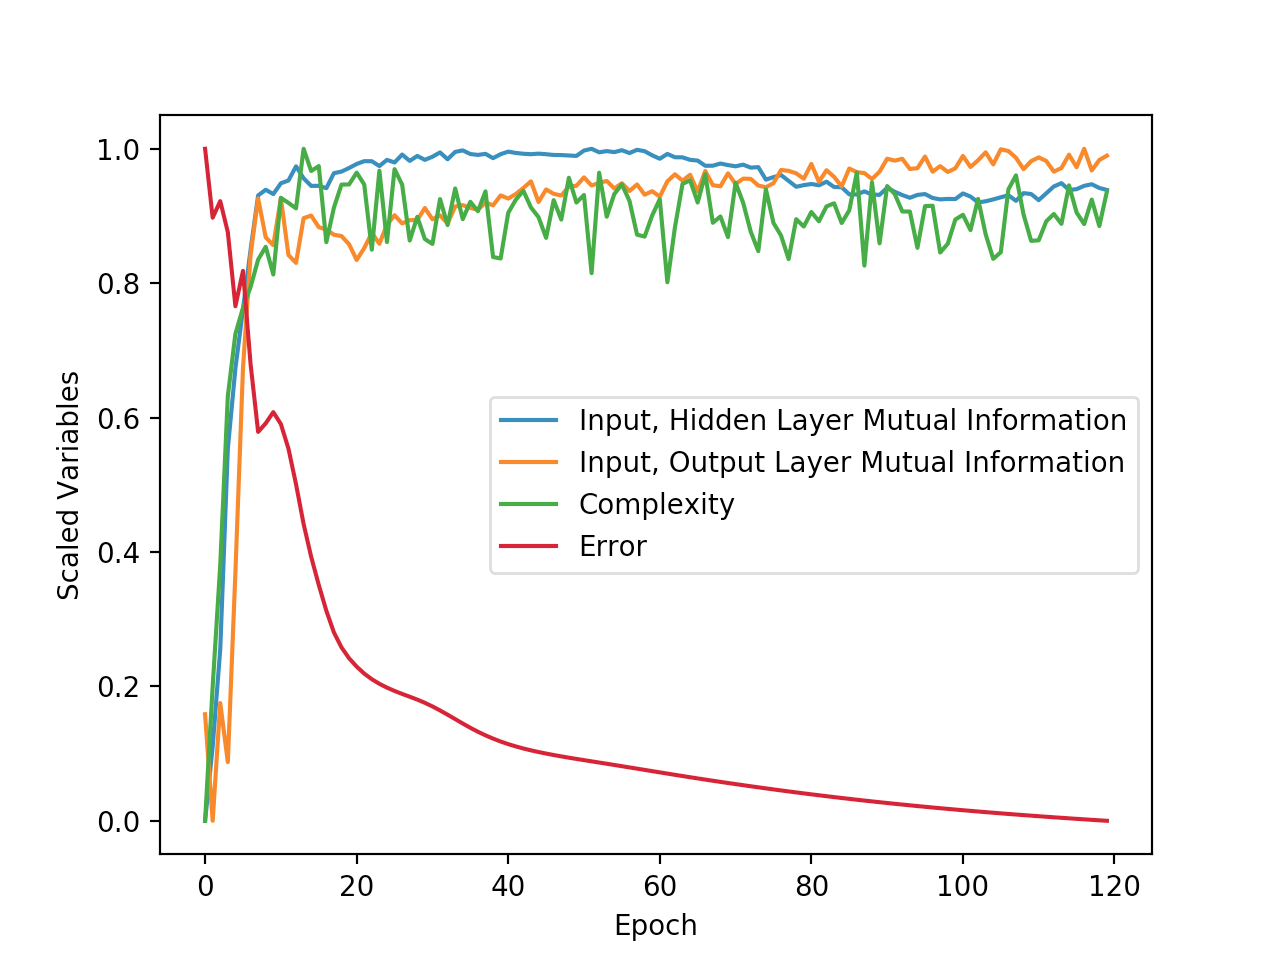
\includegraphics[width=8cm]{RNN_Images/19}
\centering
\caption{The Effective Learning Indicators}%
\end{figure}

 \section{Other Minor Results}

 In this section, we will report results which are either not very interesting or completely inconclusive. Therefore, this section will not be particularly interesting, and mostly exists to prevent the reader from thinking ''why didn't they try to do this'' on ideas we have tried.

 We analyzed how the mean the standard deviation of the gradient changes during training. As stated in ''Opening the black box of Deep Neural Networks via Information'', if the information bottleneck principle applies, we should see two distinct phases to the gradients behavior. This is not what we see. Instead we see the mean and standard deviation both approach zero with the mean always remaining (at least) slightly higher than the standard deviation.

 We tried using time delayed mutual information instead of information flow for our information flow graph, and this yielded unsatisfactory results (as expected). We tried using a ranking algorithm which utilizes the precise information flow values rather than using a threshold. That algorithm took quite a while to ''perfect'' and ended up being somewhat successful, however, due to being a bit noisy, it was less successful than our original ranking algorithm. This noise was due to there being very many pairs of neurons with (low but not negligable) information flow caused by noise.

We tried several different applications of normalizing the information flow data using entropy (to remove the effect of some neurons simply having more information than others), however, none of these yielded sufficient improvements to justify the modification. We tried analyzing the correlation between the rank of neurons and many mutual information information related statistics, but found no sufficiently interesting results.

We created some code to more objectively measure how well our ranking algorithm was doing at placing the inputs before the hidden neurons before the outputs (rather than us just judging by the look of the histograms). This yielded no non-obvious results. We did some analysis of the rates of change of the activations of all the neurons, and found nothing substantial.

 \section{Conclusion}

 Fully recurrent neural networks have very chaotic and difficult to follow behavior. Analyzing information flow graphs is potentially a good way to understand the structure, however, they are rather difficult to interpret. Our ranking algorithm is potentially another useful tool, however, it requires a large amount of neurons to find statistically significant results (aside from simple results we already know a priori)  and is still somewhat difficult to interpret. Despite this, their results have been shown to be valid in that they show the inputs have lower rank than the hidden neurons which have lower rank than the output.

 Their is no indication that the information bottle neck principle applies to our fully recurrent neural network. However, it is still unknown whether this is a fluke of our neural network, or if the information bottleneck principle simply doesn't apply to fully recurrent neural networks. The mutual information between the output and the hidden neurons for our network behaves in an odd way during training that neither fits the information bottleneck principle nor the more basic idea of the mutual information always increasing.

After training (during testing), the mutual information of neurons with the input is positively correlated with the mutual information of neurons with the output. This most likely indicates that some neurons are more important than others, and that this effect overwhelms the fact that some neurons store more information about the input and some neurons store more information about the output. The idea of mutual information statistics being a useful indicator of learning certainly applies to fully recurrent neural networks. Specifically, the mutual information with the input and the TSE complexity are good learning indicators.

\section{Future Work}

The most obvious piece of future work is trying to re-test our conclusions with other recurrent neural networks. Specifically, we would like to test if the information bottleneck principle applies to other recurrent neural networks (because us finding negative results here was somewhat surprising).

In my opinion, the most important and difficult piece of future work is finding better ways to analyze the information flow graph. I believe the information flow graph is a great starting point for analyzing recurrent neural networks. However, it is a difficult starting point simply due to the problem of understanding neural networks being very challenging. However, it is still possible that the information flow graph is mostly random and chaotic (aside from containing the ranking information we found in this paper), rather than just being very difficult to interpret. If that is true (which would surprise me), an additional piece of future work would be designing a new method of analyzing the way information flows in the network.

Another piece of future work is applying the ranking algorithm to larger networks, and applying more tests of the effectiveness of the ranking algorithm. Applying the ranking algorithm to larger networks could help show if their are patterns in the ranking (as explained earlier in this paper). To further test the validity of the ranking algorithm, it could be applied to a feed forward neural network to see how well it mimics the desired results (having the rank of a neural be proportional to the layer that neuron is in).

It would also be interesting to perform a more rigorous analysis of learning indicators. For example, one could analyze how the learning indicates behave under various situations where the network is not set up correctly (not set up in a way in which it will successfully learn). This could be used to see if learning indicators provide useful diagnostics for ''debugging'' neural networks. I believe the next step for learning indicators is showing how the network is learning (and revealing flaws in the learning) rather than just showing if the network is learning.


\nocite{ntnu}
\nocite{black_box}
\nocite{weather}
\nocite{disentangling_representations}
\nocite{info_bottleneck}
\nocite{rnn_time_series}
\nocite{rnn_stocks}
\nocite{speech}
\nocite{text}
\nocite{mutual_info}
\nocite{content_transfer}
\nocite{social_media}

\bibliographystyle{unsrt}
\bibliography{references}


\end{document}